\chapter{Extending the Line of Action to Multiple Characters}\label{chap:implementation}

\section{Approach}
Almost inverting the problem at hand, we start from a pose to find the appropriate lines of action by tracing over the shapes of the dancers' bodies using the Grease Pencil Tool in Blender. It was carried out with the purpose of clarifying the properties and limitations of the typical line of action. After seeing at which point the actions started to repeat, a shorter sub-clip was chosen. Annotation was performed in five different ways:
\begin{enumerate}
	\item tracking and marking each characters' contact with the ground
	\item tracking and marking each characters' contact with each other
	\item tracing lines of action for each character separately every few frames, using the previous line of action notation -- the baseline method.
	\item tracing lines of action for the characters and treating them as one using as few strokes as possible every few frames.
	\item once the main common combinations were established from the above two methods, tracing lines of action only for the selected extreme combination poses.
\end{enumerate}

\begin{figure}[h!]
	\centering
        \begin{subfigure}[b!]{0.45\textwidth}
        	\centering
                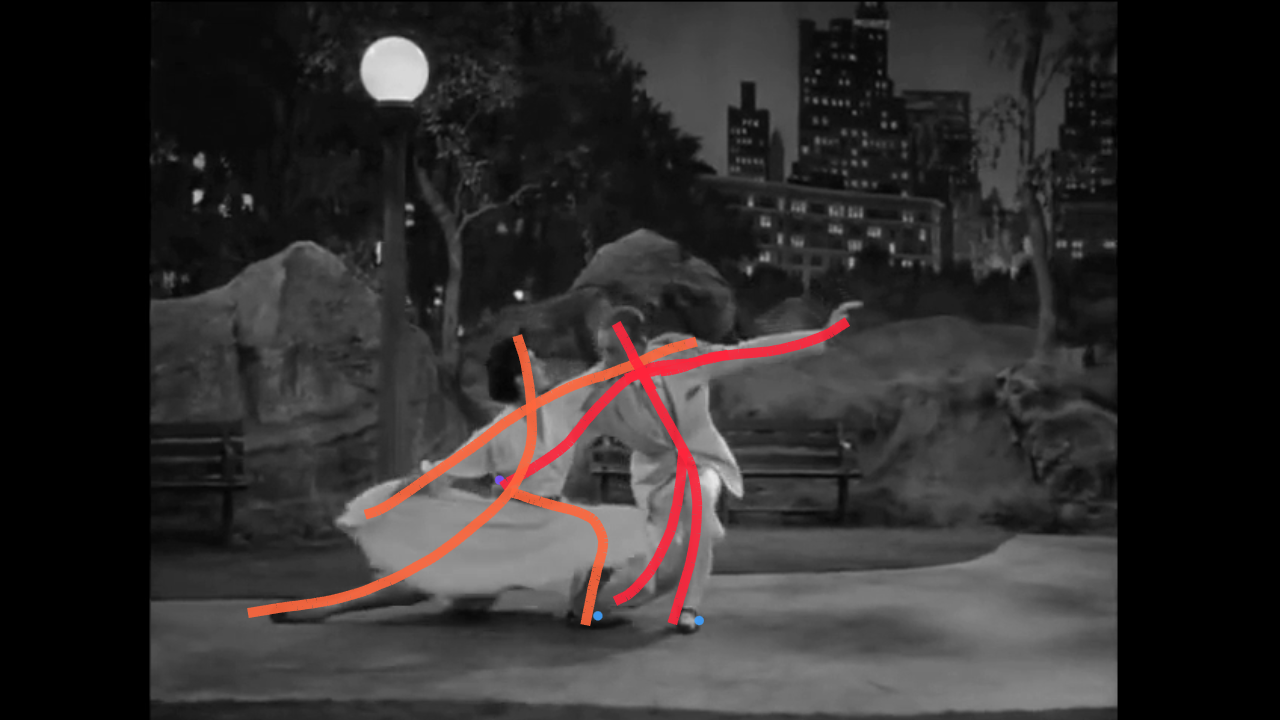
\includegraphics[width=\linewidth]{img/keyframe_case_7_baseline}
                \caption{The typical lines of action trace out the whole skeleton, and in the worst case is 3 lines per character.}
                \label{fig:baseline}
        \end{subfigure}
        \quad
        \begin{subfigure}[b!]{0.45\textwidth}
        	\centering
                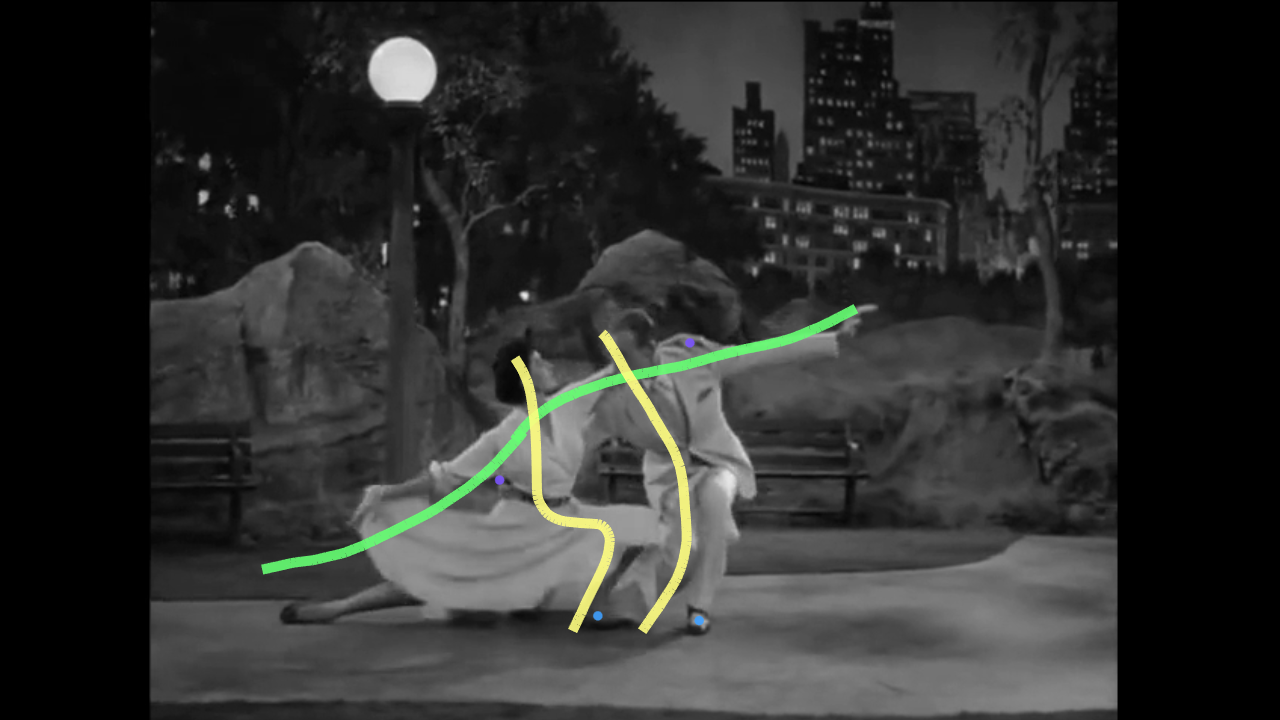
\includegraphics[width=\linewidth]{img/keyframe_case_7_new}
                \caption{Treating the characters as one bigger character allows the user to draw fewer lines to indicate the same pose.}
                \label{fig:new_notation}
        \end{subfigure}%
        \caption{Comparing the old line of action and the new.}
	\label{fig:poses}
\end{figure}

Through this process, certain patterns and common poses stood out, enabling the development of an improved notation for illustrating the poses of characters during their interactions with each other. Patterns included symmetry, parallelism, and repetition. Of course, using these patterns and assumptions to our advantage is what drove the development of a solution. It seemed that during many instances in the clip, it would be more efficient to draw lines over the two dancers as if they were one character. This morphed ``combined'' character should be easier to pose and animate.

\begin{figure}[h!]
	\centering
        \begin{subfigure}[b!]{0.45\textwidth}
        	\centering
                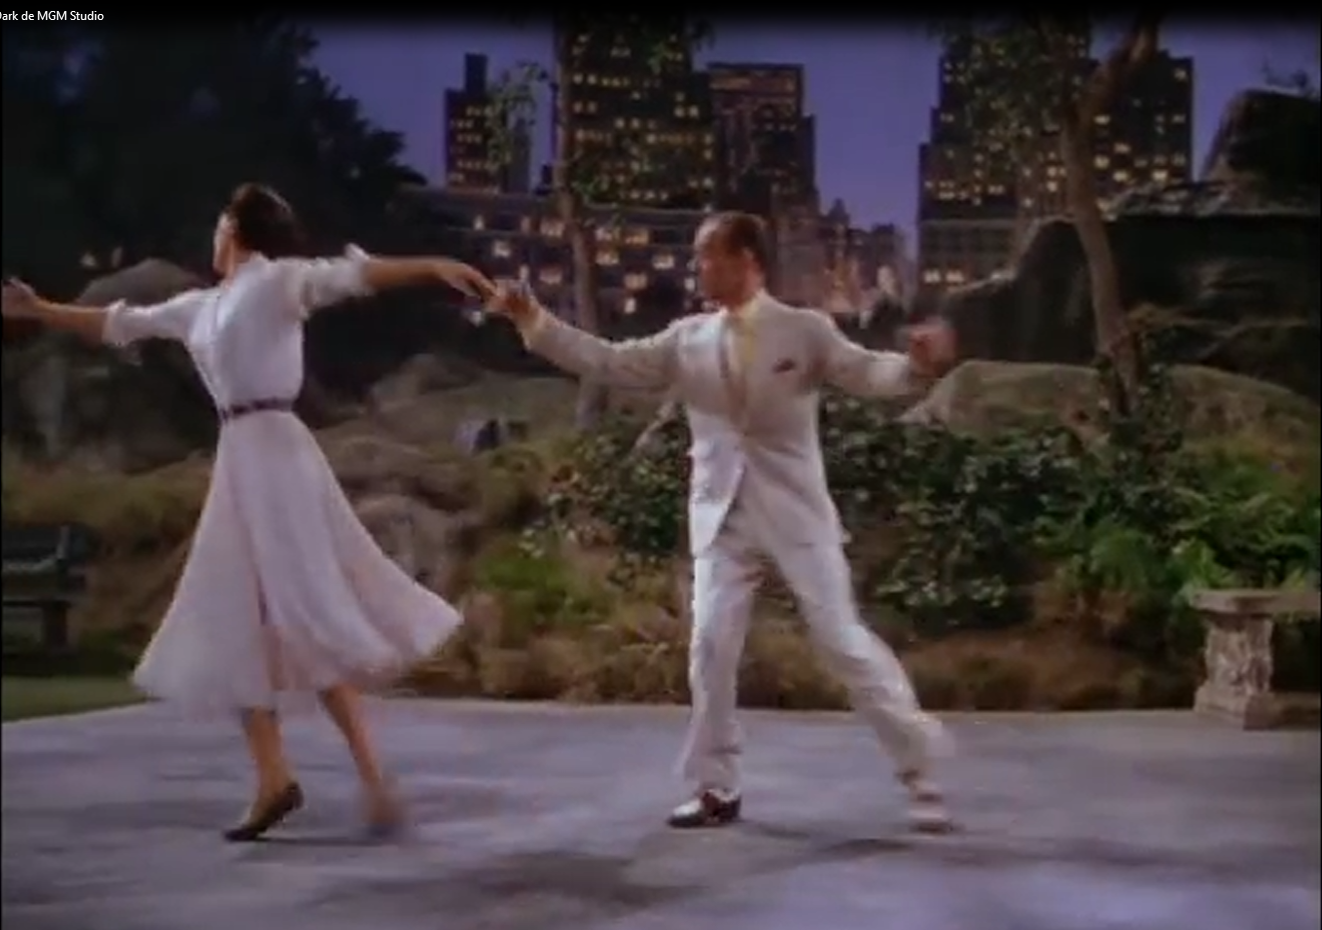
\includegraphics[width=\linewidth]{img/parallelism}
                \caption{Parallelism.}
                \label{fig:parallelism}
        \end{subfigure}
        \quad
        \begin{subfigure}[b!]{0.45\textwidth}
        	\centering
                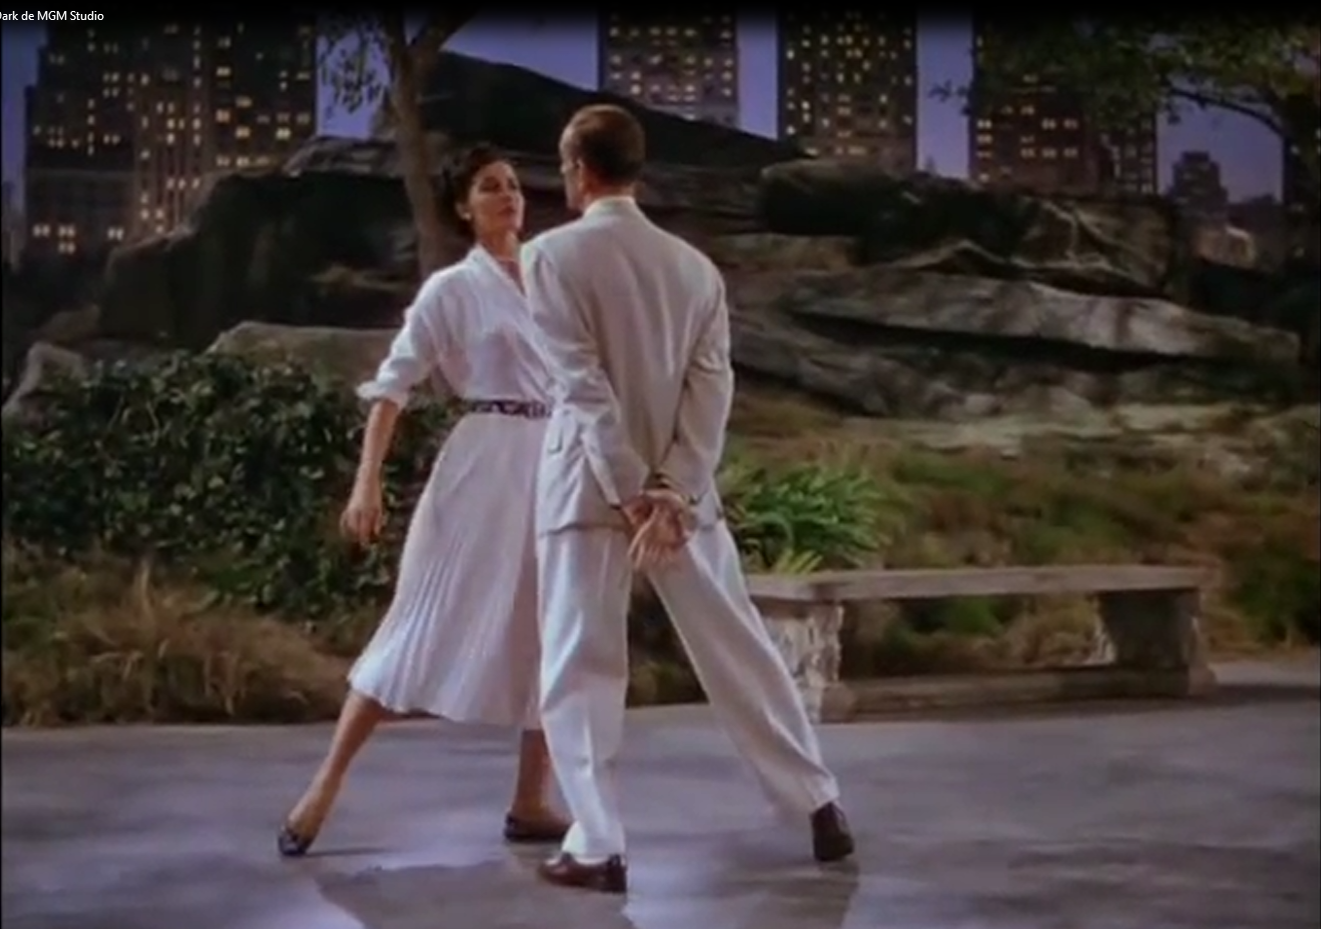
\includegraphics[width=\linewidth]{img/symmetry}
                \caption{Symmetry.}
                \label{fig:symmetry}
        \end{subfigure}%
        \caption{Patterns in the poses.}
	\label{fig:patterns}
\end{figure}

\begin{figure}[h!]
	\centering
        \begin{subfigure}[b!]{0.31\textwidth}
        	\centering
                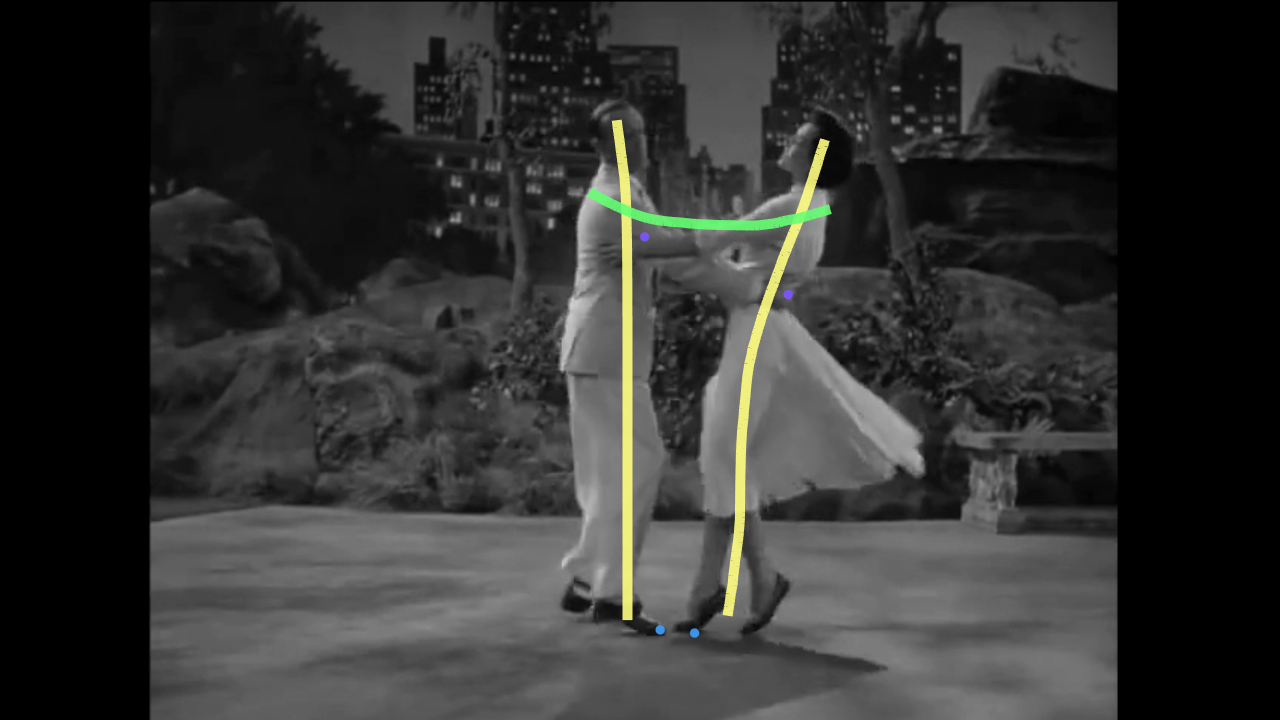
\includegraphics[width=\linewidth]{img/keyframe_case_4_(3)}
                \label{fig:pose1}
        \end{subfigure}
        \quad
        \begin{subfigure}[b!]{0.31\textwidth}
        	\centering
                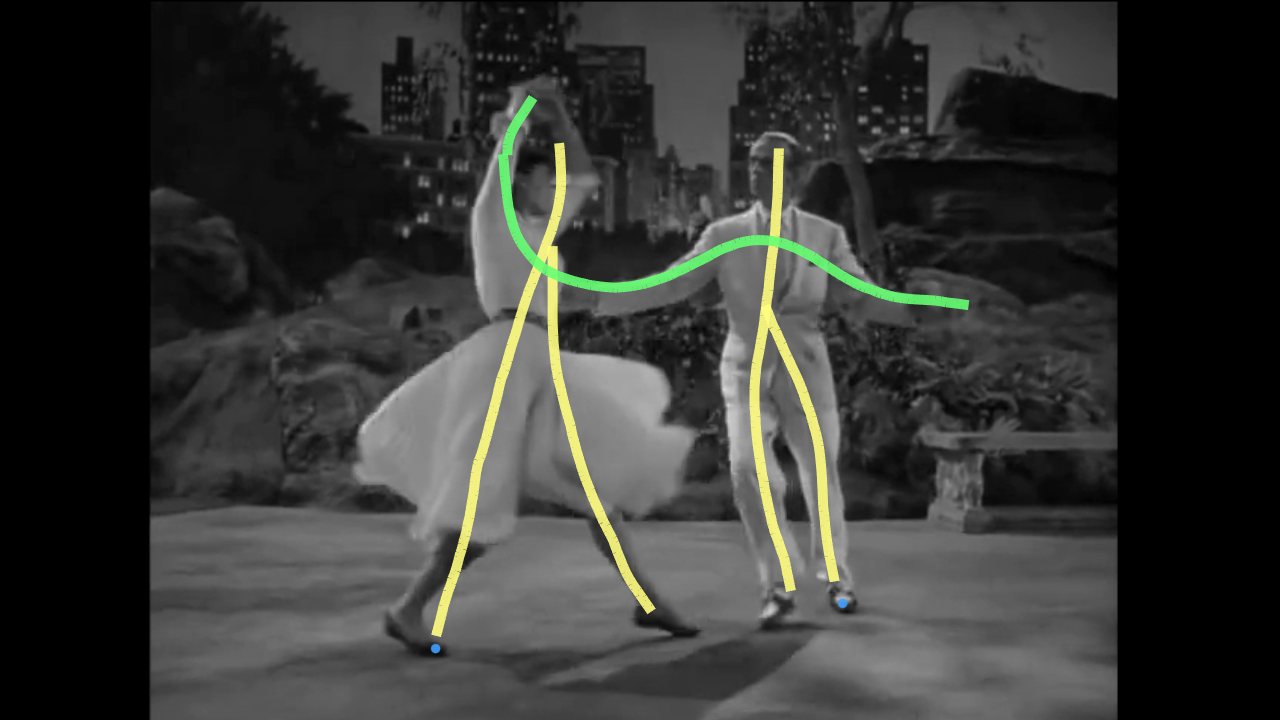
\includegraphics[width=\linewidth]{img/keyframe_case_10_(5)}
                \label{fig:pose2}
        \end{subfigure}%
        \quad
        \begin{subfigure}[b!]{0.31\textwidth}
        	\centering
                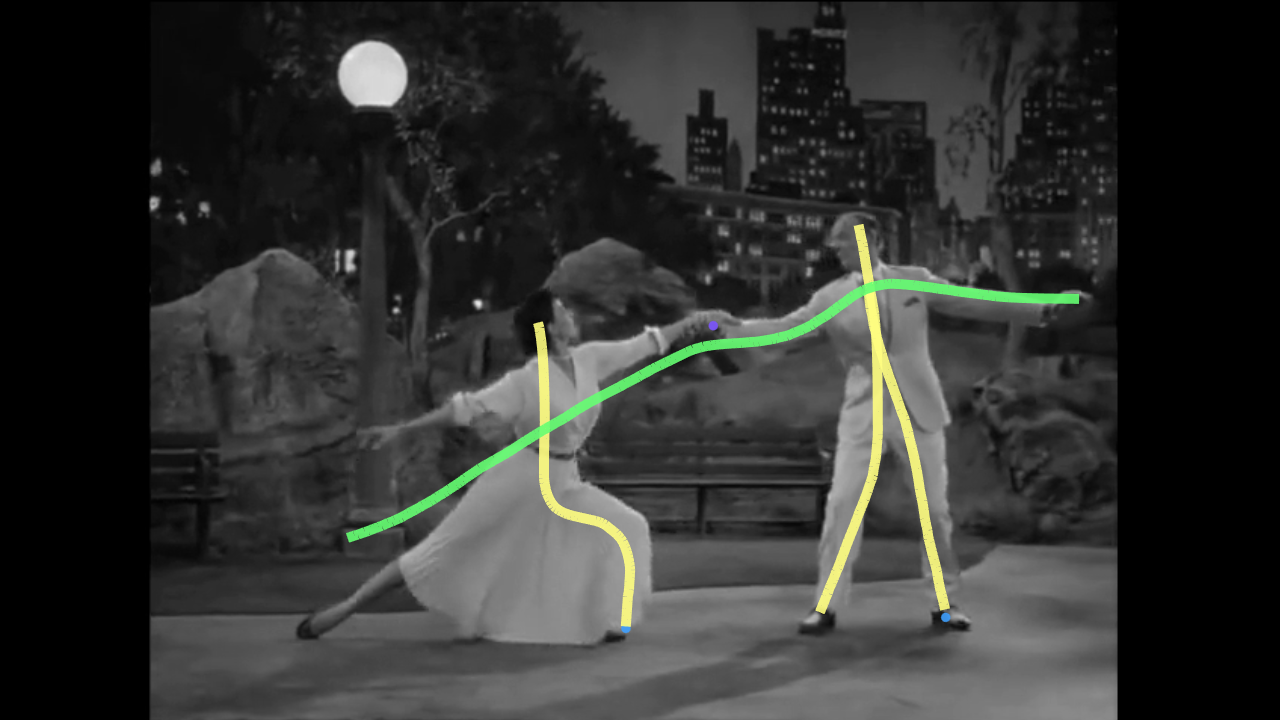
\includegraphics[width=\linewidth]{img/keyframe_case_7_(4)}
                \label{fig:pose3}
        \end{subfigure}%
	\caption{A selection of tracings over the dance clip from ``The Band Wagon.''}
	\label{fig:tracing}
\end{figure}

\section{Interface}


\section{Merging Kinematics Trees}
Rather than changing the whole LOA concept and optimization algorithm, we reduce the more complex problem of using LOAs on multiple characters to the original LOA problem and utilize (nearly) the exact same minimization.

\citep{johnson1975finding}

\subsection{Notation}
Taking inspiration from Sutton Notation, we propose a new notation for representing the poses of two characters both together and separately.

\subsubsection{Common Multi-character Poses}
\begin{wrapfigure}{L}{0.55\textwidth}
\centering
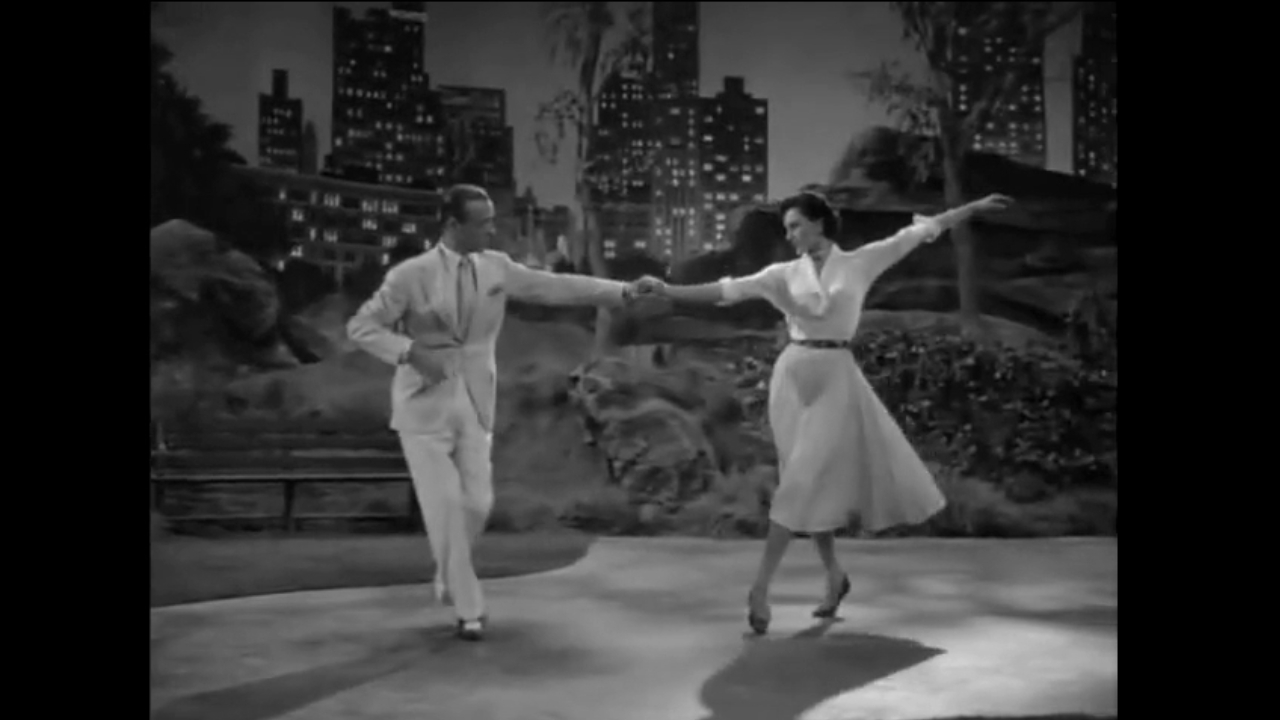
\includegraphics[scale=0.1]{img/bandwagon}
\caption{Dancing in the Dark.}
\end{wrapfigure}

There is a dance scene in the film ``The Band Wagon,'' where Cyd Charisse and Fred Astaire start out by walking together side by side, exchanging twirls until it morphs completely into a swing style dance. This scene is our use case for inventing a notation which extends seamlessly to more than one character.

To determine which poses for these dancers were common, I annotated the video with what I thought good keyframes would be if the two characters were treated as one. 

\begin{table}[!htb]
  \centering
  \begin{tabular}{ | c | c || c | c | c | }
    \hline
     & Separate & \multicolumn{3}{c |}{Together}\\ \hline
    1 LOA 
    & &
    \begin{minipage}{.15\textwidth}
      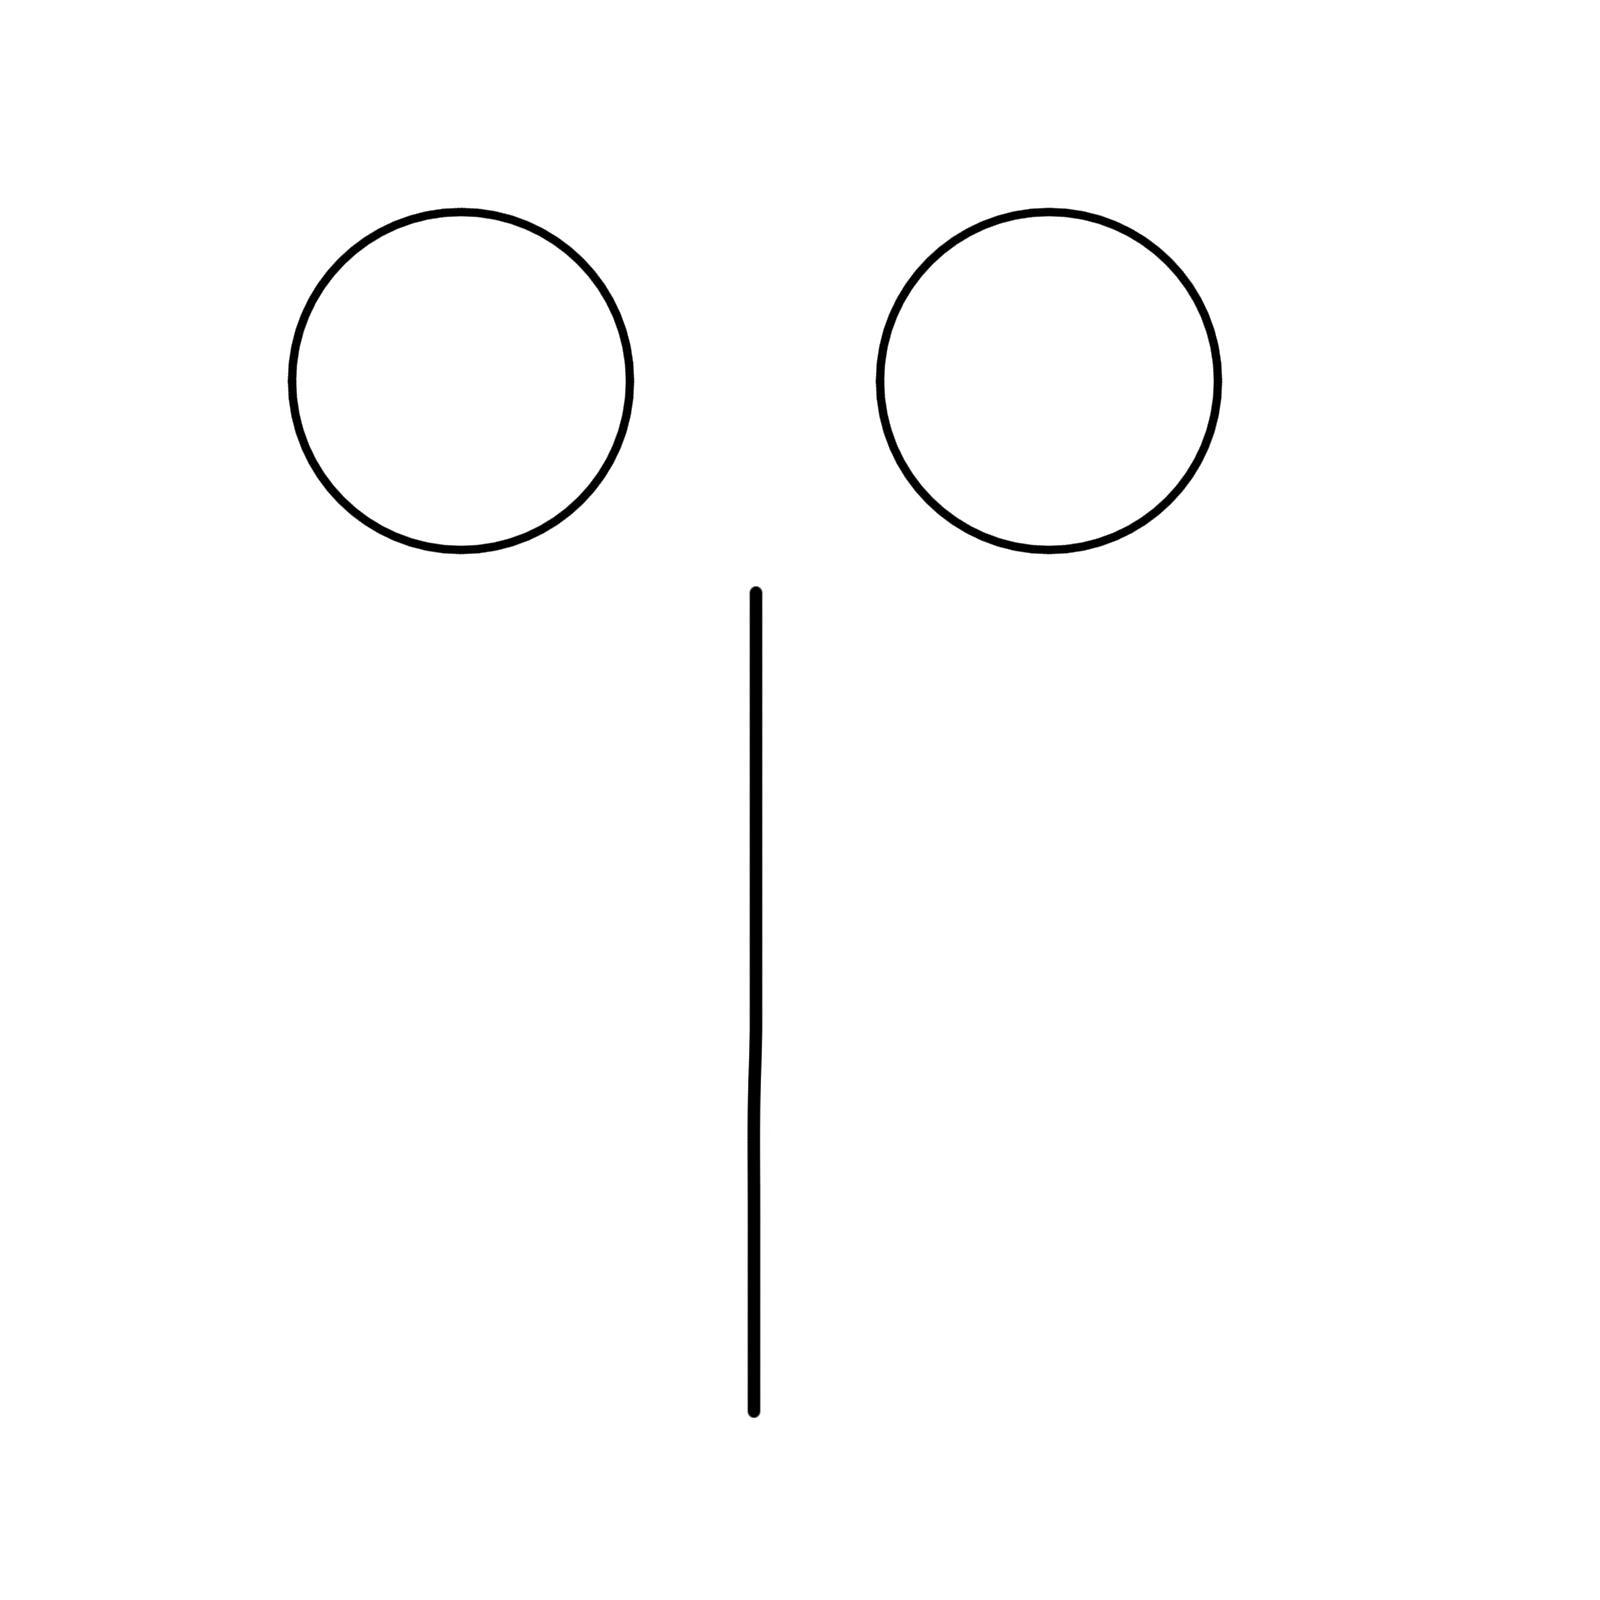
\includegraphics[width=\linewidth, height=20mm]{img/01keyframe}
    \end{minipage} & & \\ 
    \hline
    2 LOA 
    &
    \begin{minipage}{.15\textwidth}
      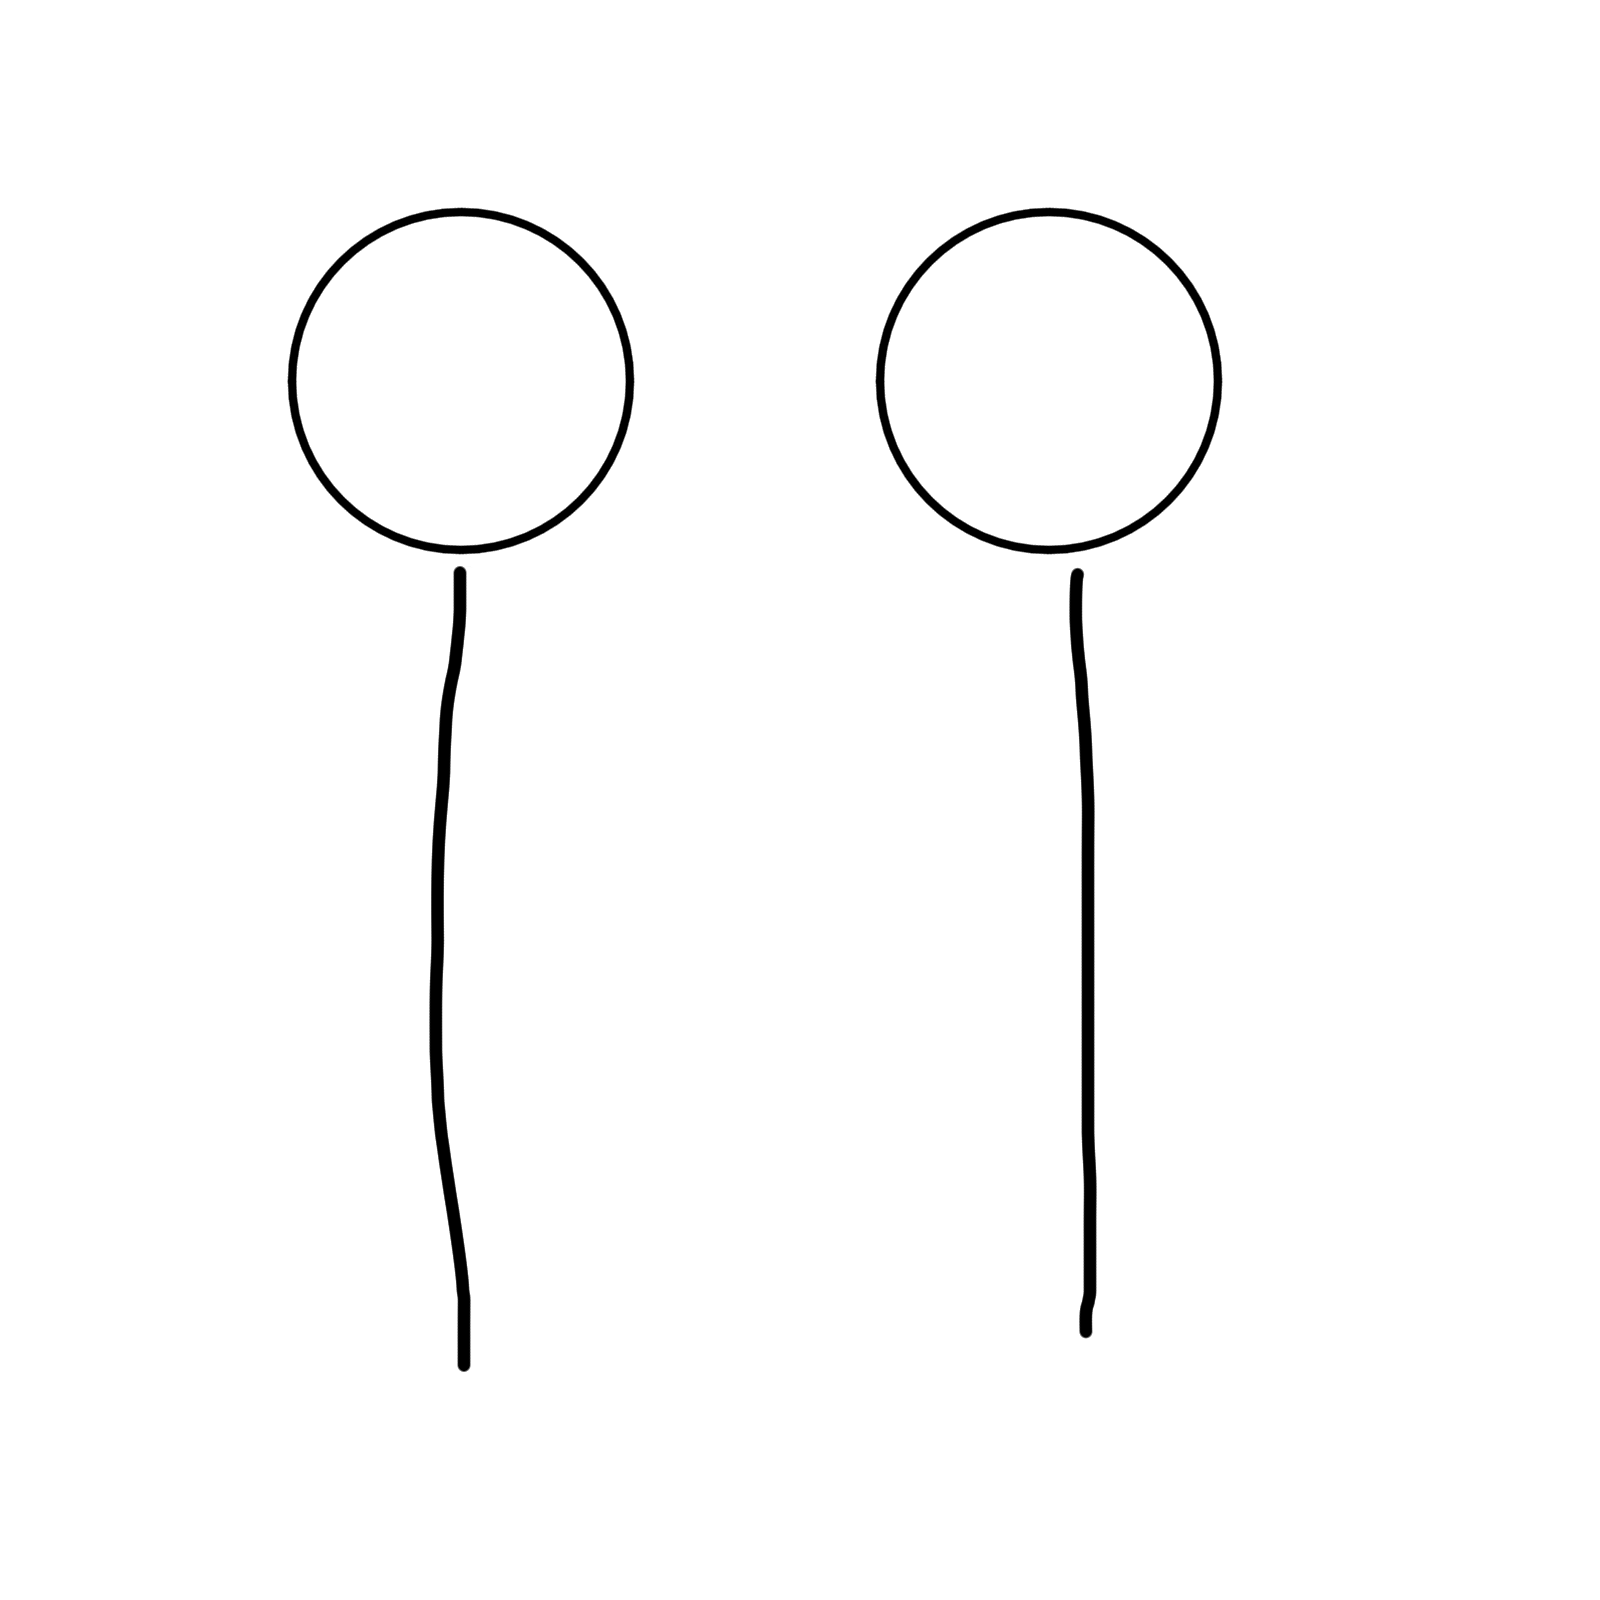
\includegraphics[width=\linewidth, height=20mm]{img/2loa_separate_keyframe}
    \end{minipage}
    &
    \begin{minipage}{.15\textwidth}
      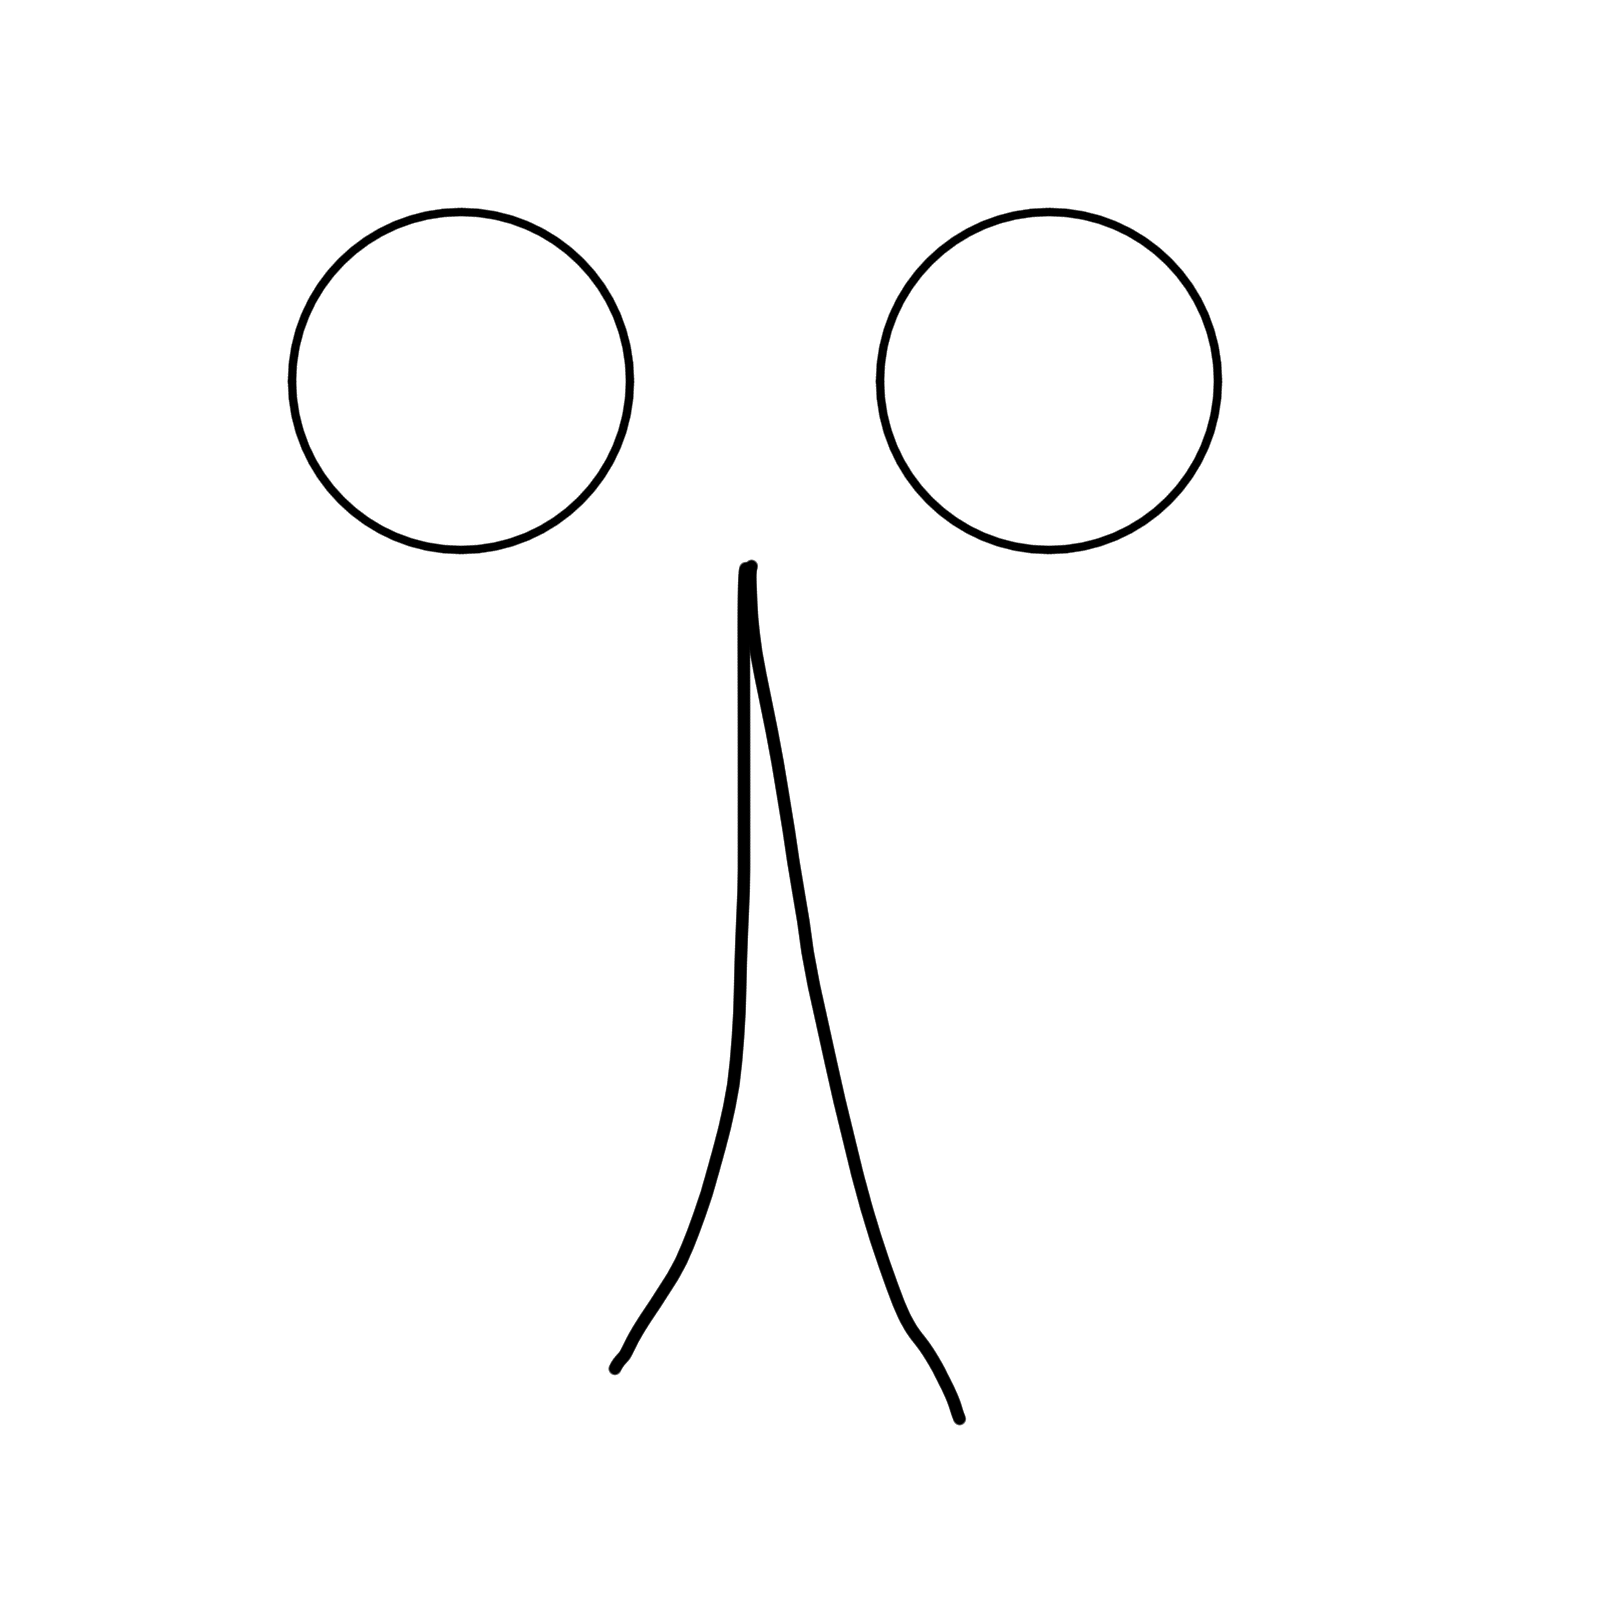
\includegraphics[width=\linewidth, height=20mm]{img/02keyframe}
    \end{minipage}
    &
    \begin{minipage}{.15\textwidth}
      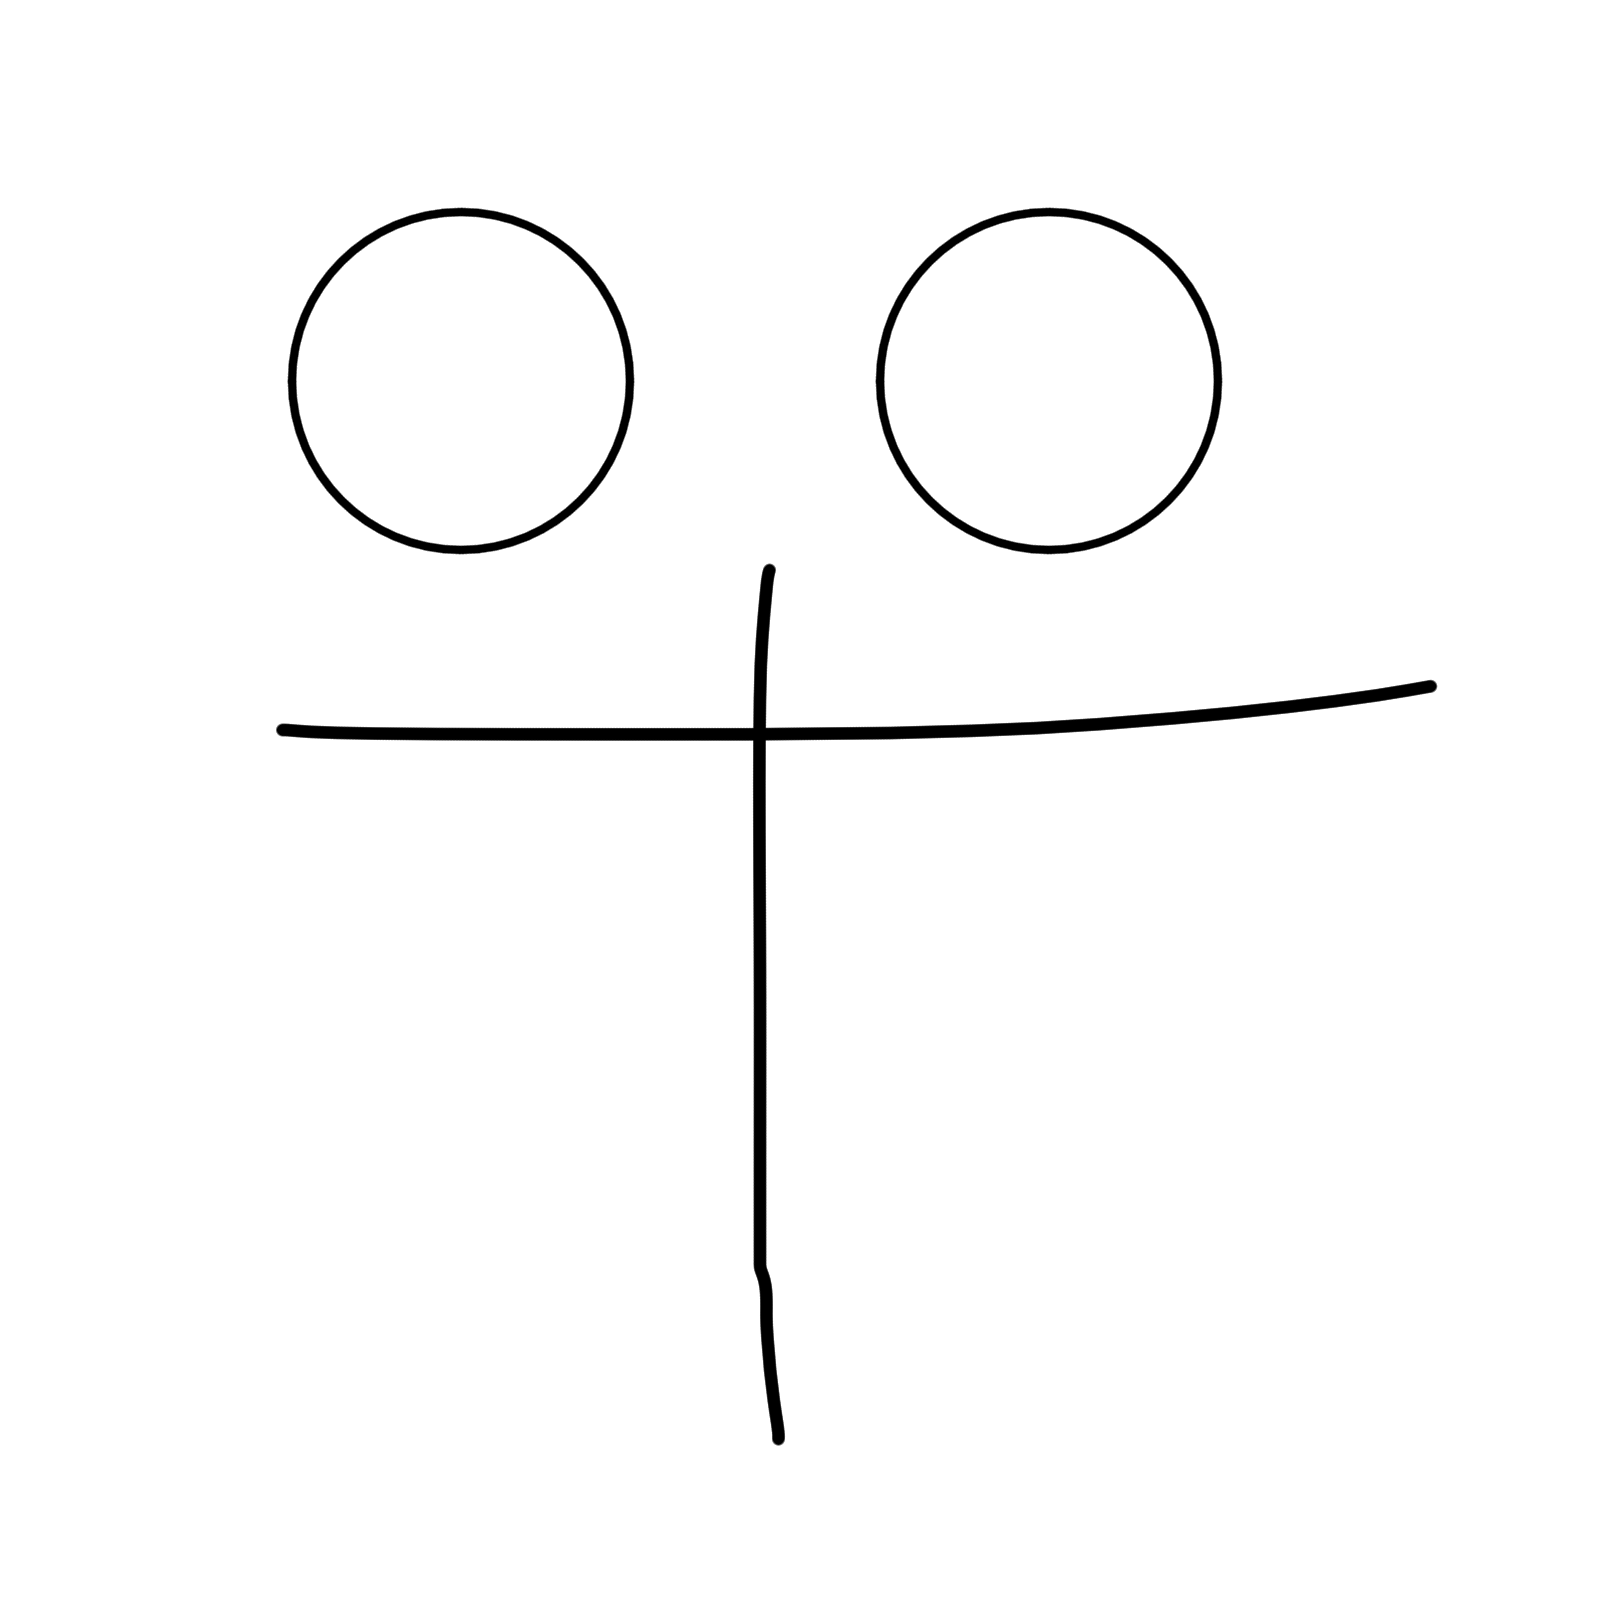
\includegraphics[width=\linewidth, height=20mm]{img/03keyframe}
    \end{minipage} & 
    \\ \hline
    3 LOA 
    &
    \begin{minipage}{.15\textwidth}
      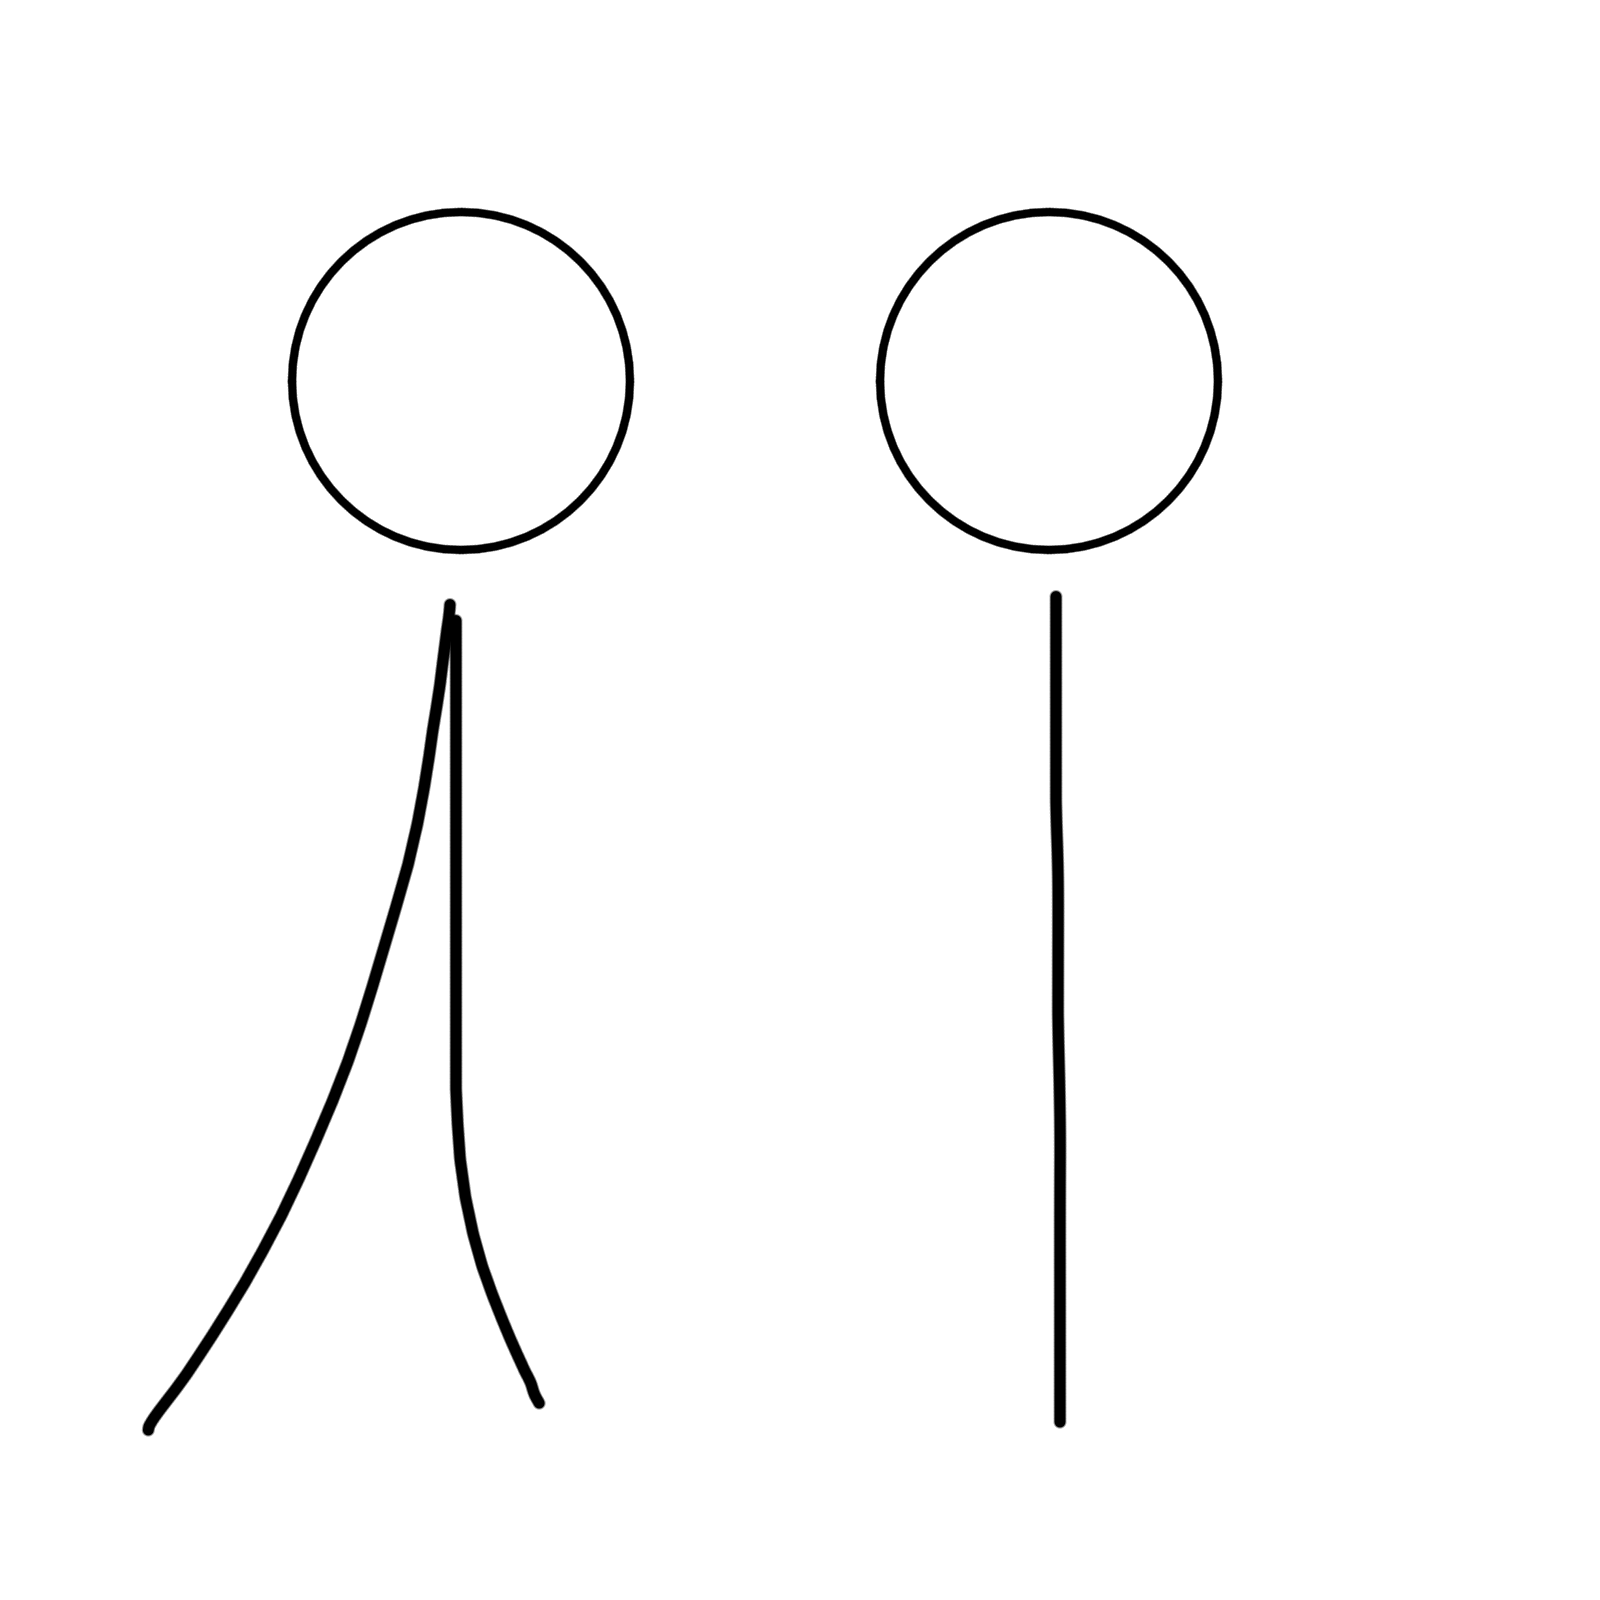
\includegraphics[width=\linewidth, height=20mm]{img/3loa_separate_keyframe}
    \end{minipage}
    &
    \begin{minipage}{.15\textwidth}
      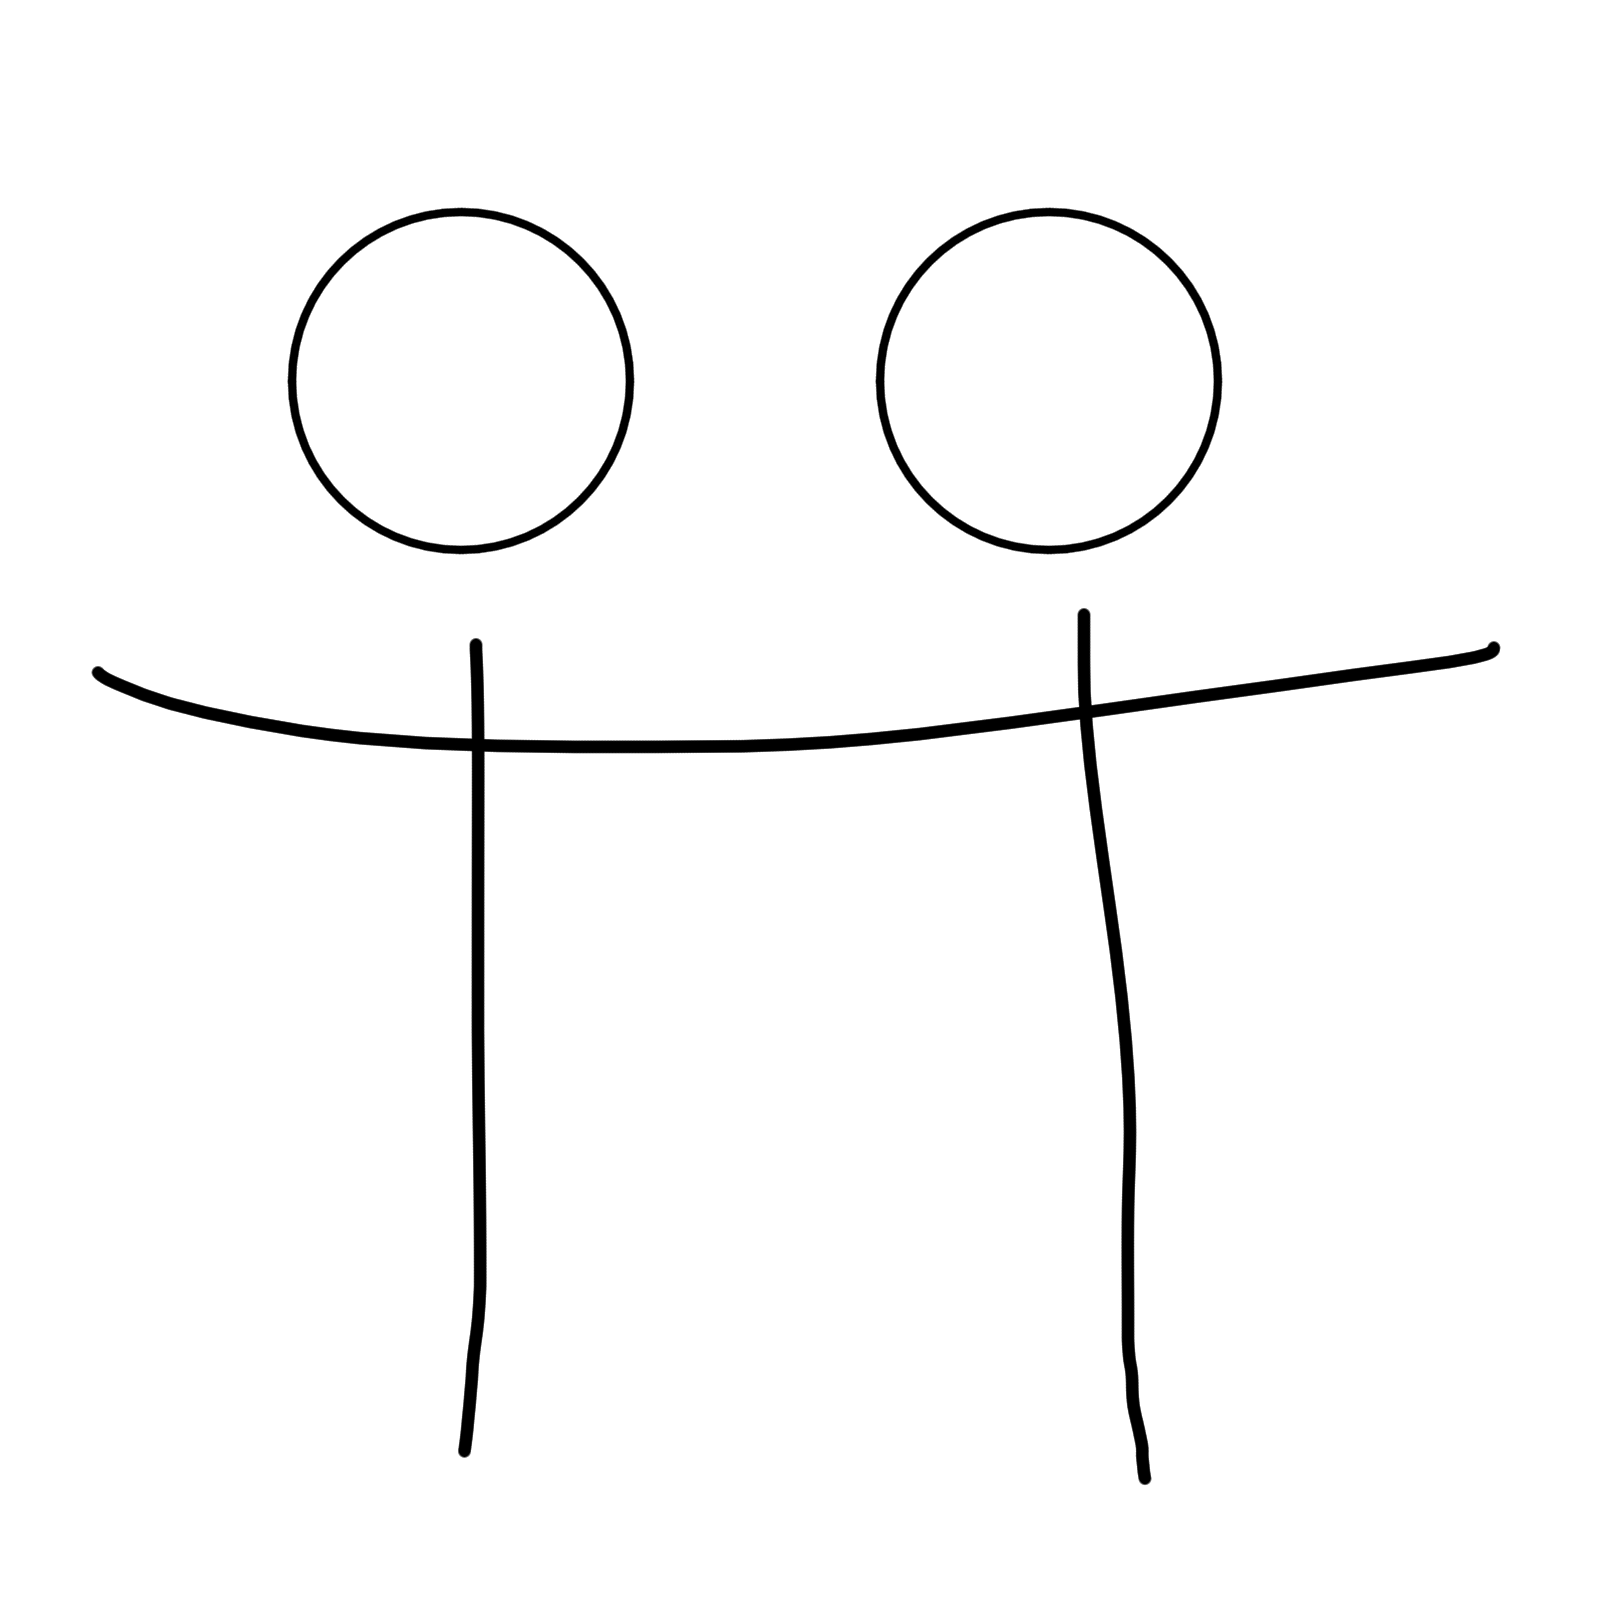
\includegraphics[width=\linewidth, height=20mm]{img/04keyframe}
    \end{minipage}
    &
    \begin{minipage}{.15\textwidth}
      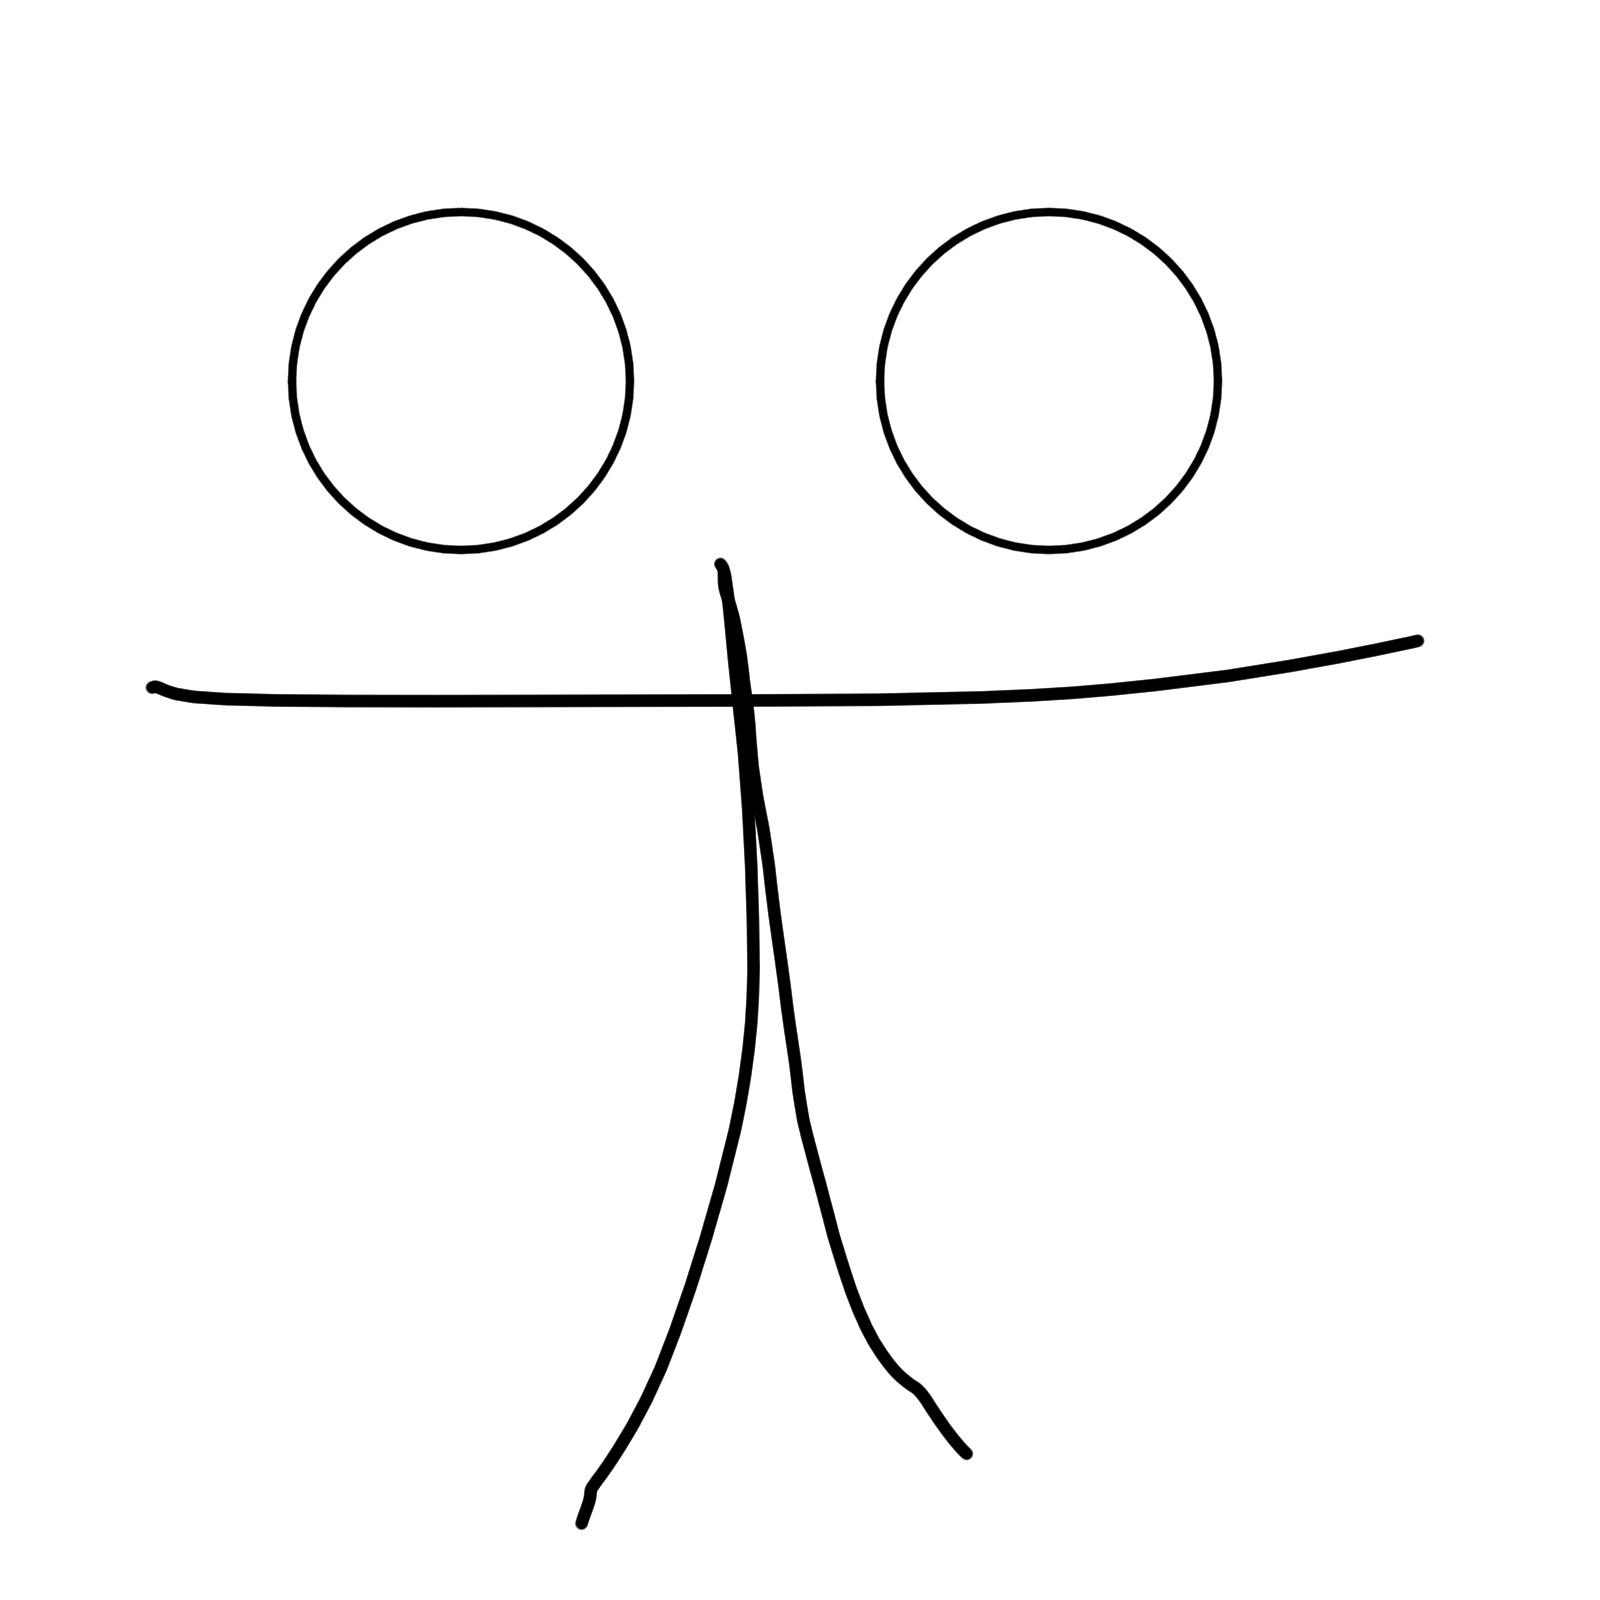
\includegraphics[width=\linewidth, height=20mm]{img/05keyframe}
    \end{minipage} 
    & 
    \begin{minipage}{.15\textwidth}
      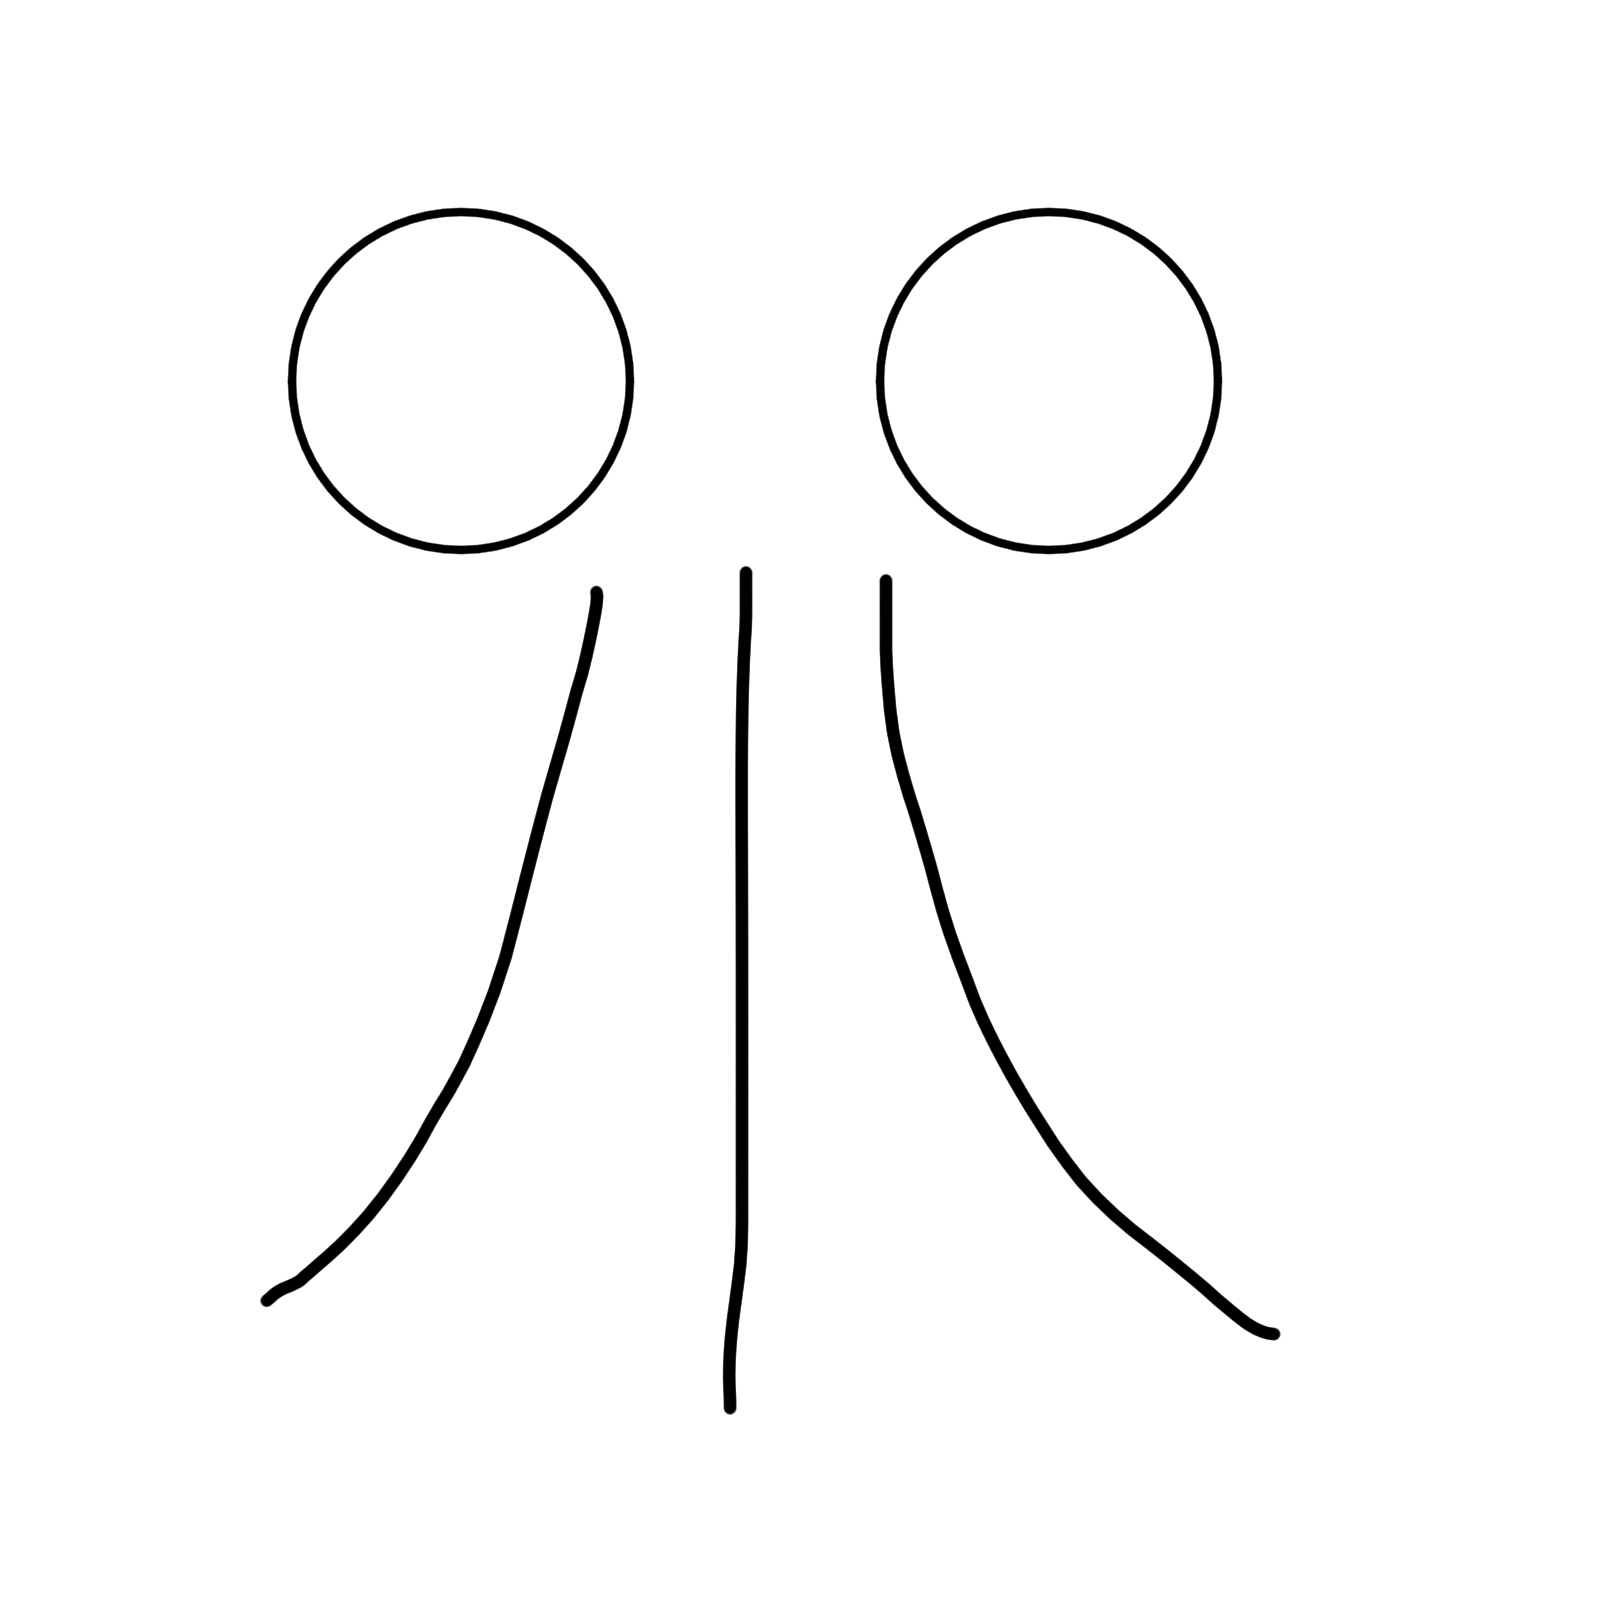
\includegraphics[width=\linewidth, height=20mm]{img/06keyframe}
    \end{minipage} 
    \\ \hline
    4 LOA 
    &
    \begin{minipage}{.15\textwidth}
      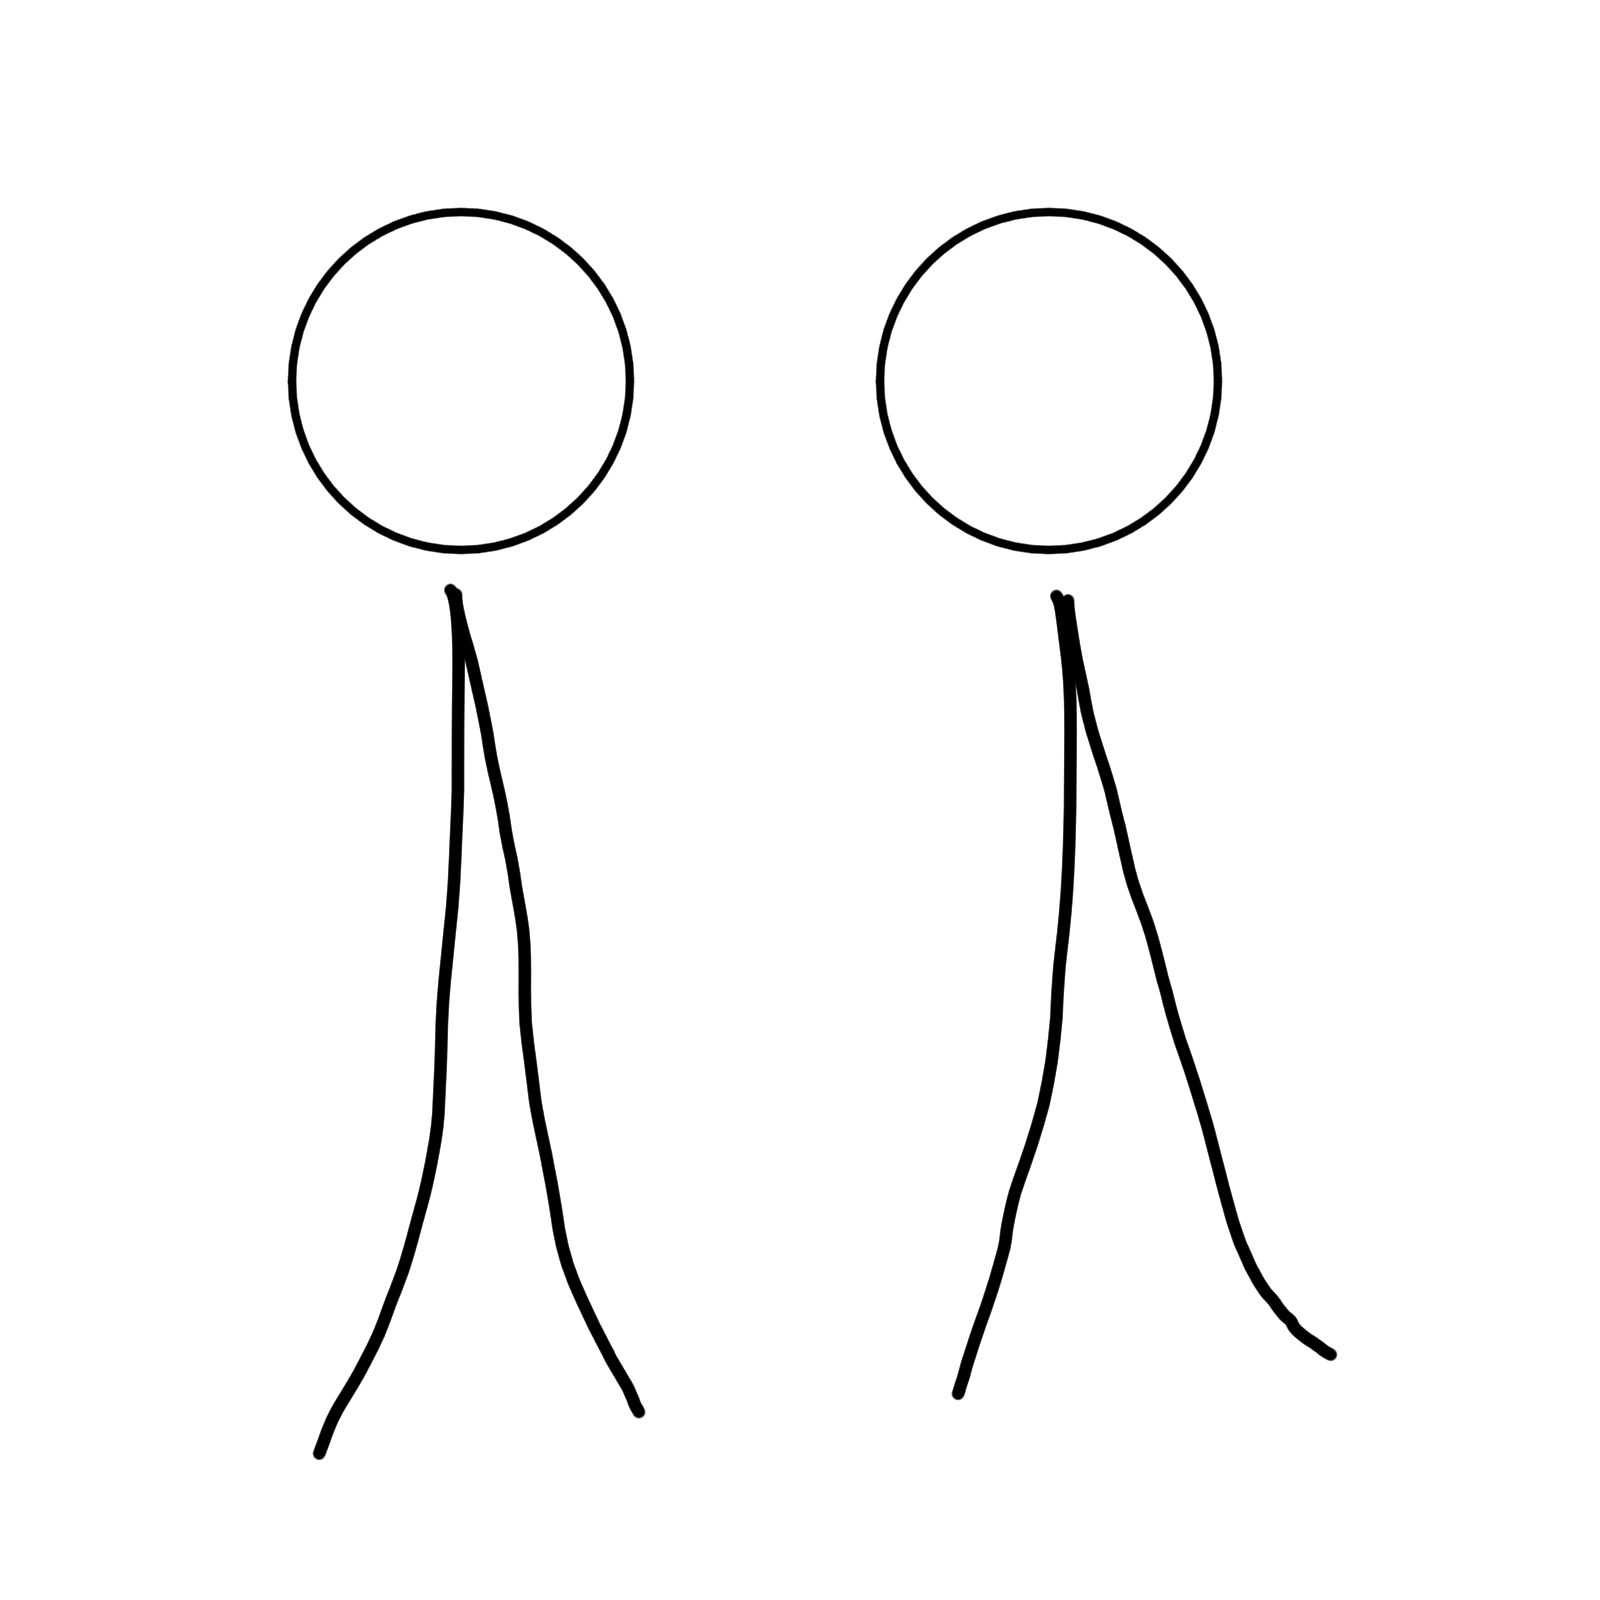
\includegraphics[width=\linewidth, height=20mm]{img/4loa_separate_keyframe}
    \end{minipage}
    &
    \begin{minipage}{.15\textwidth}
      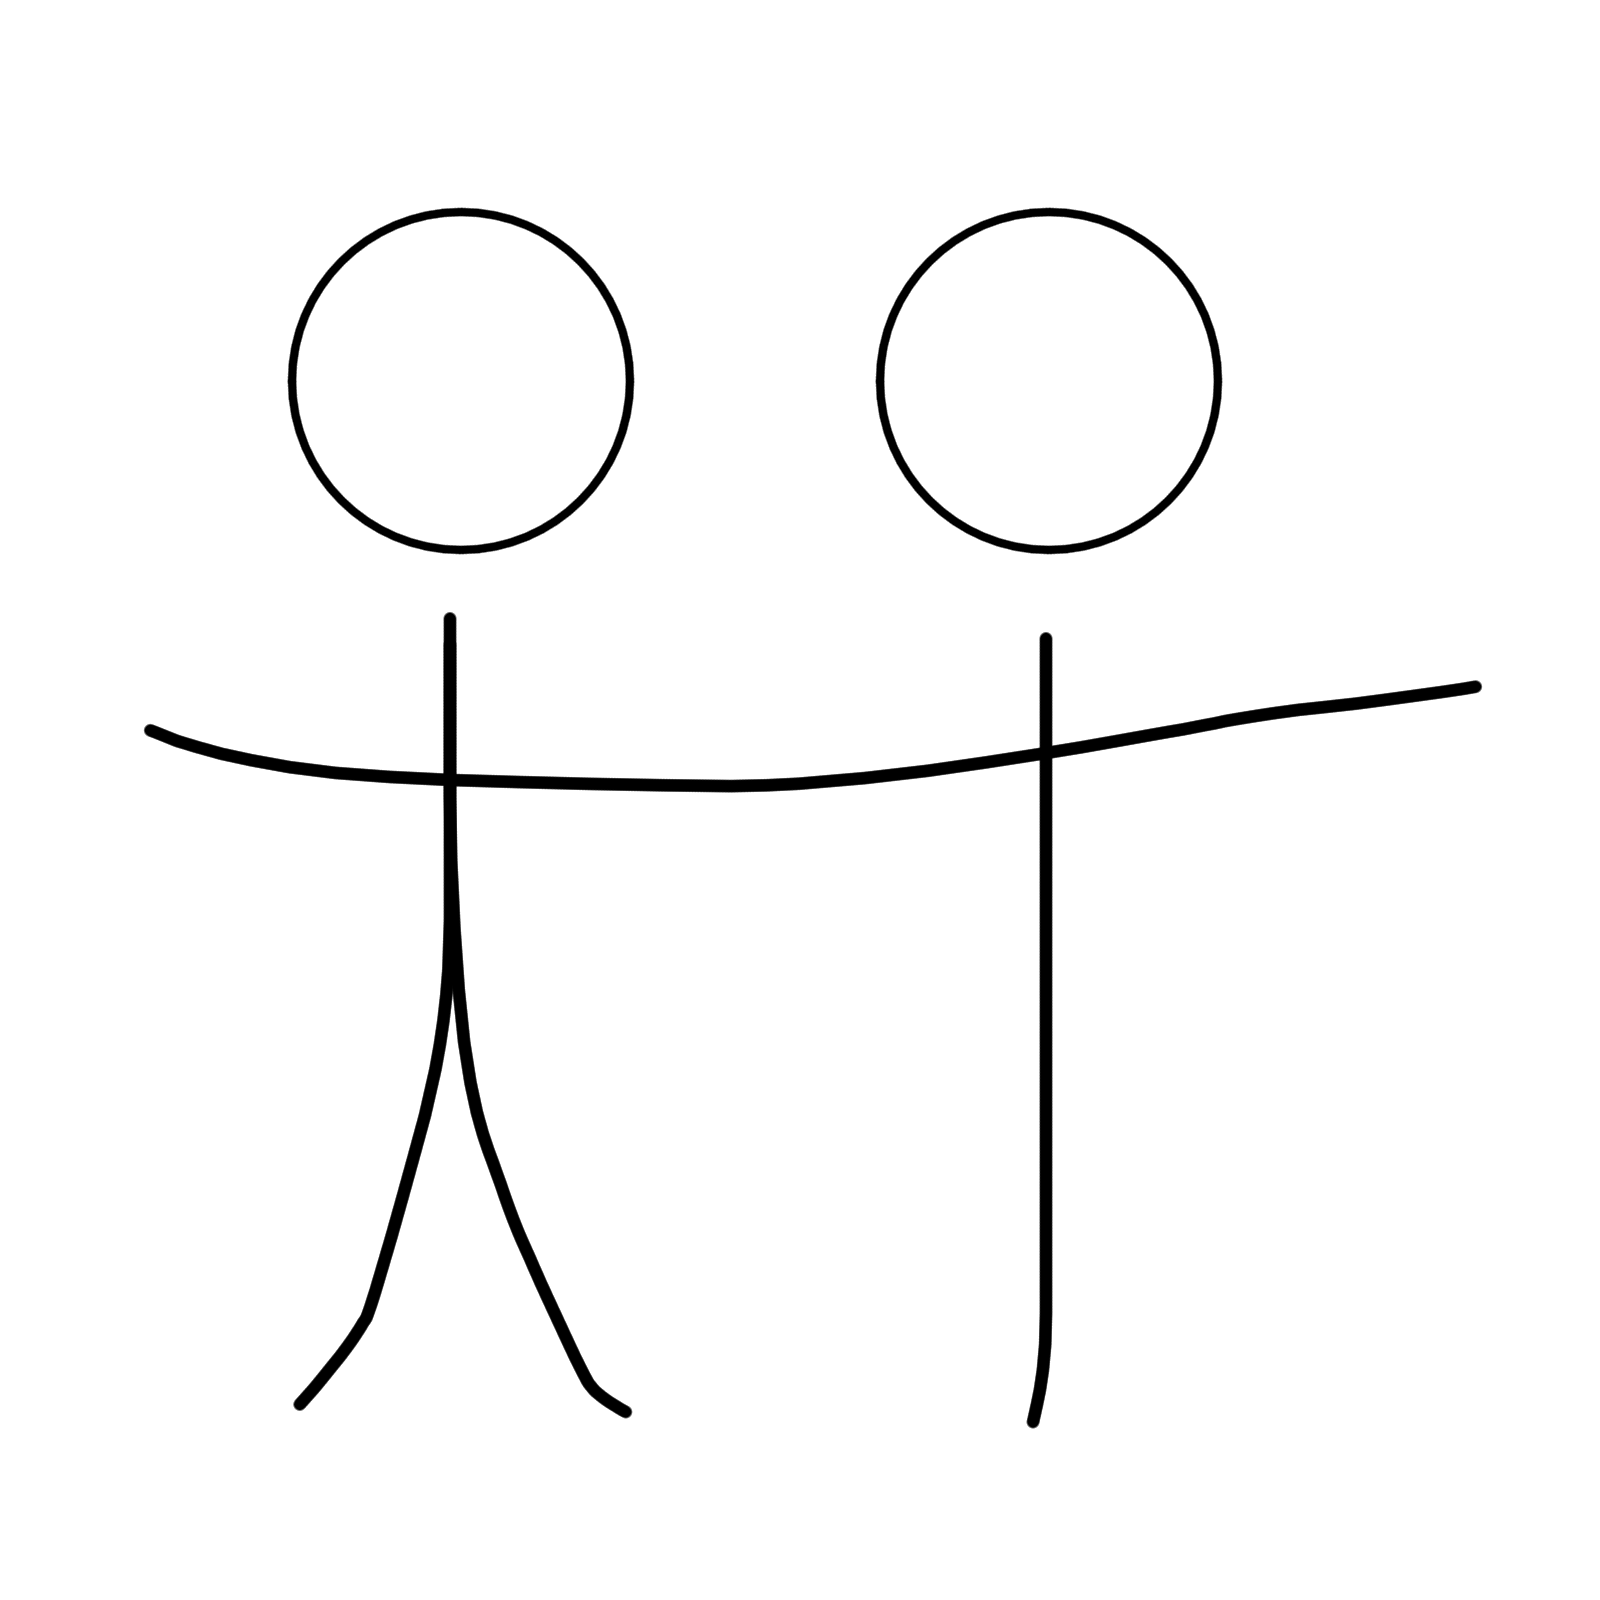
\includegraphics[width=\linewidth, height=20mm]{img/07keyframe}
    \end{minipage}
    &
    \begin{minipage}{.15\textwidth}
      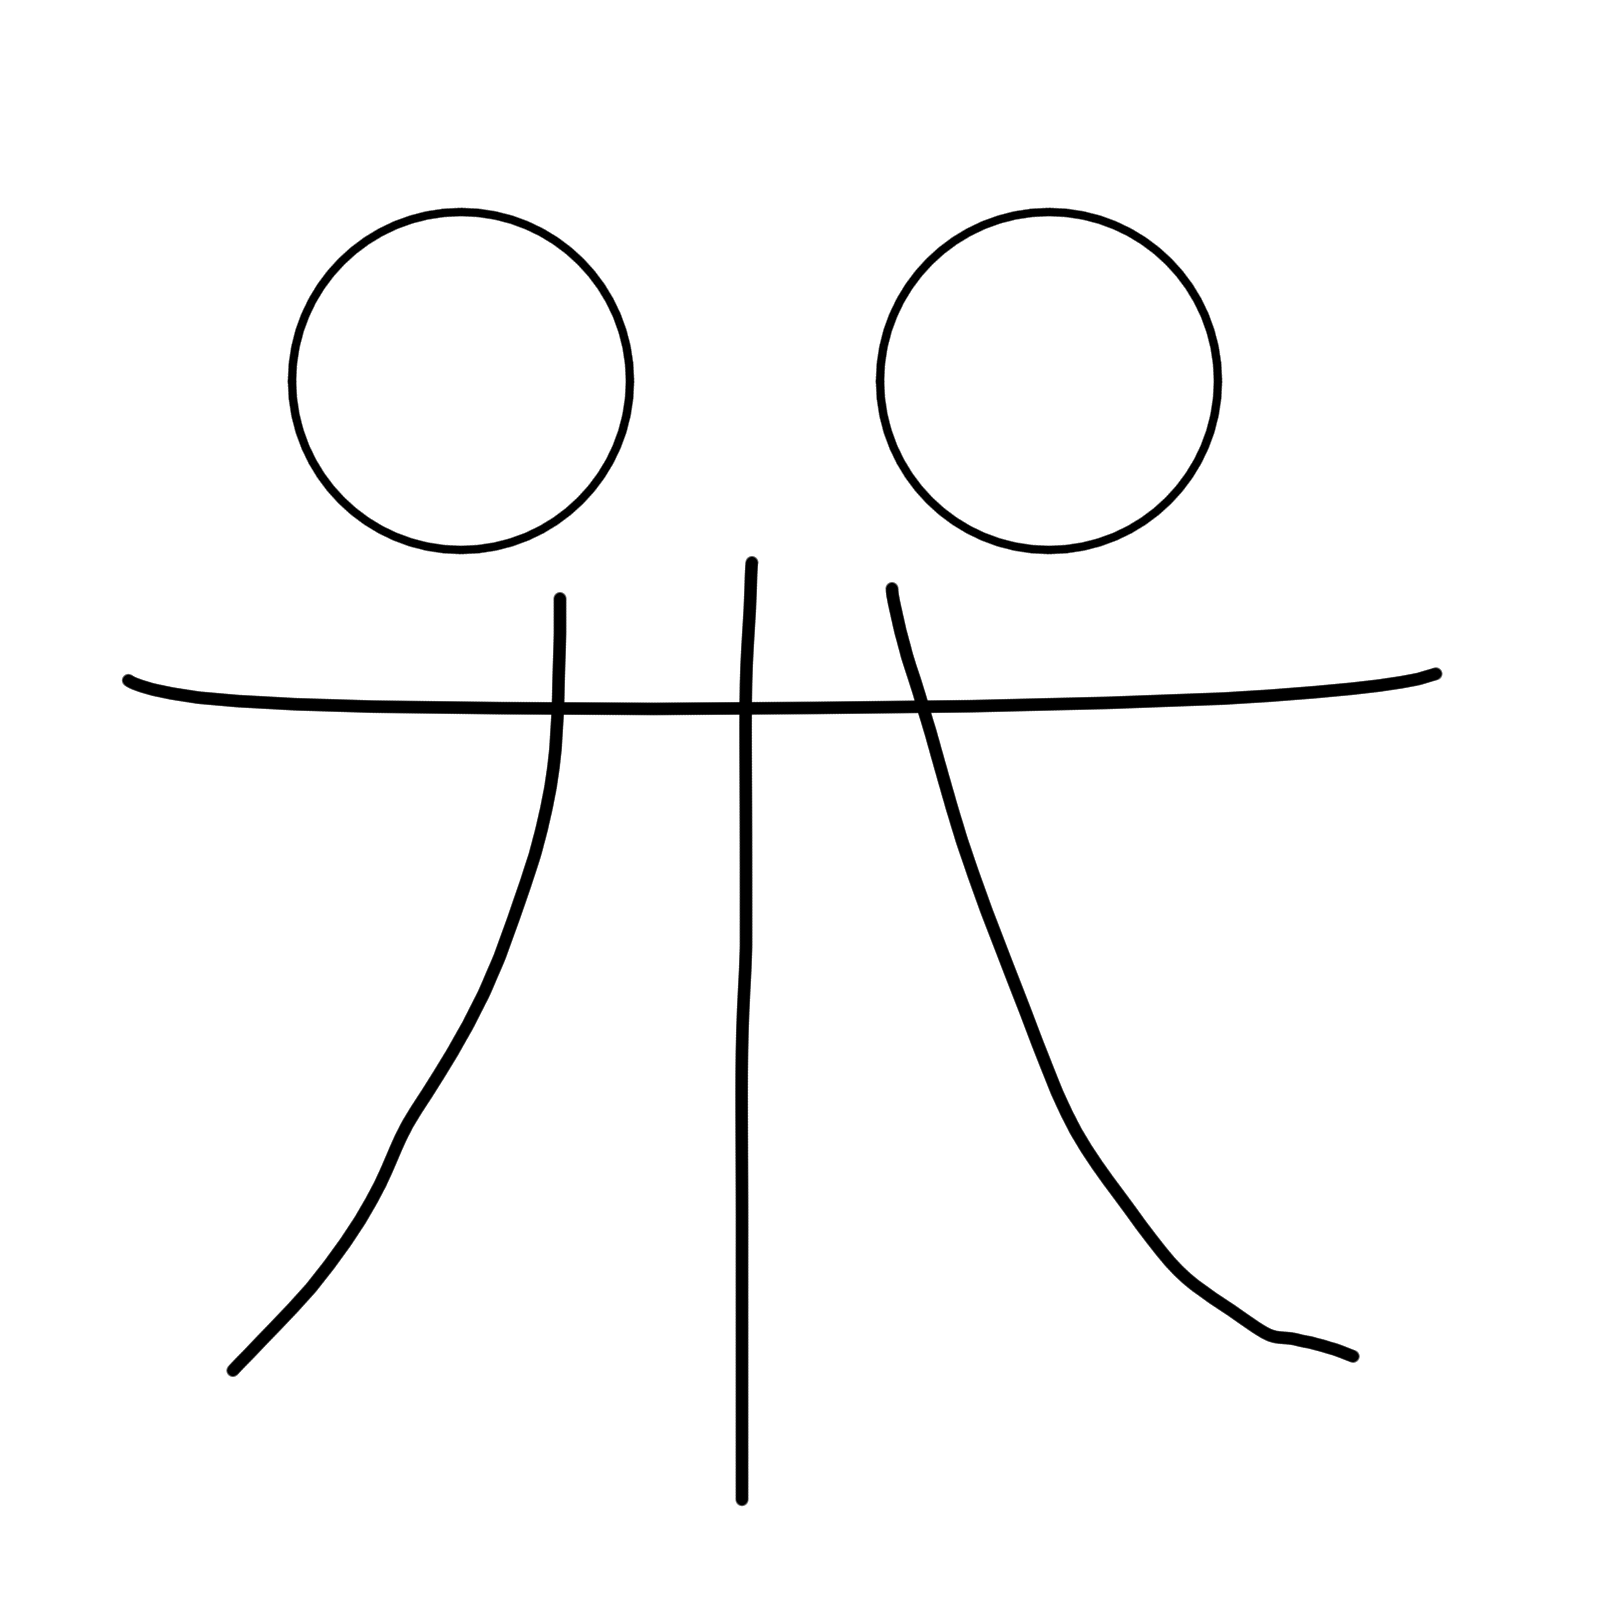
\includegraphics[width=\linewidth, height=20mm]{img/08keyframe}
    \end{minipage} 
    & 
    \begin{minipage}{.15\textwidth}
      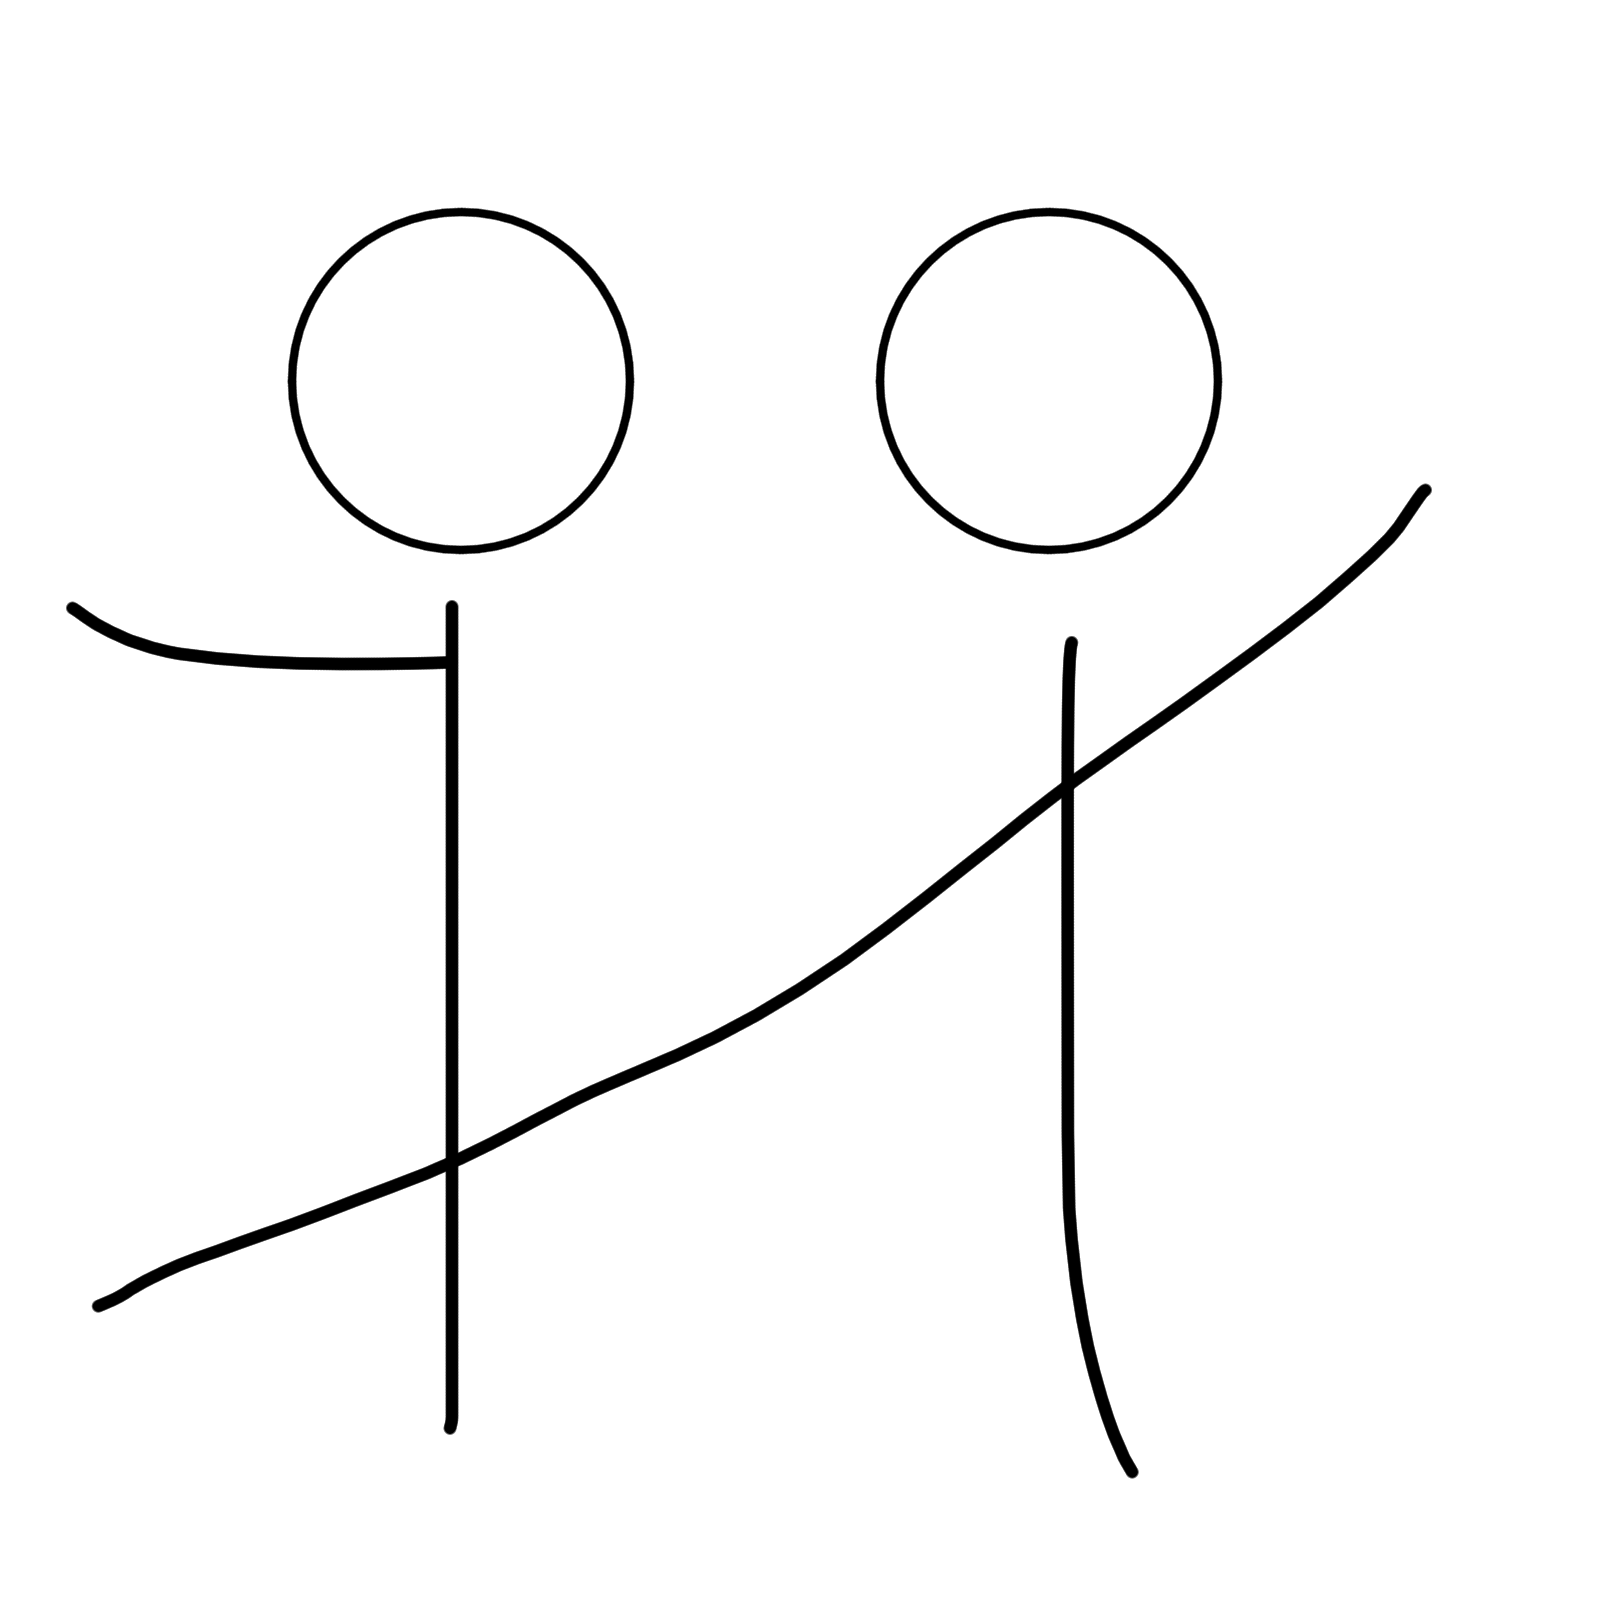
\includegraphics[width=\linewidth, height=20mm]{img/09keyframe}
    \end{minipage} 
    \\ \hline 
    &
    \begin{minipage}{.15\textwidth}
      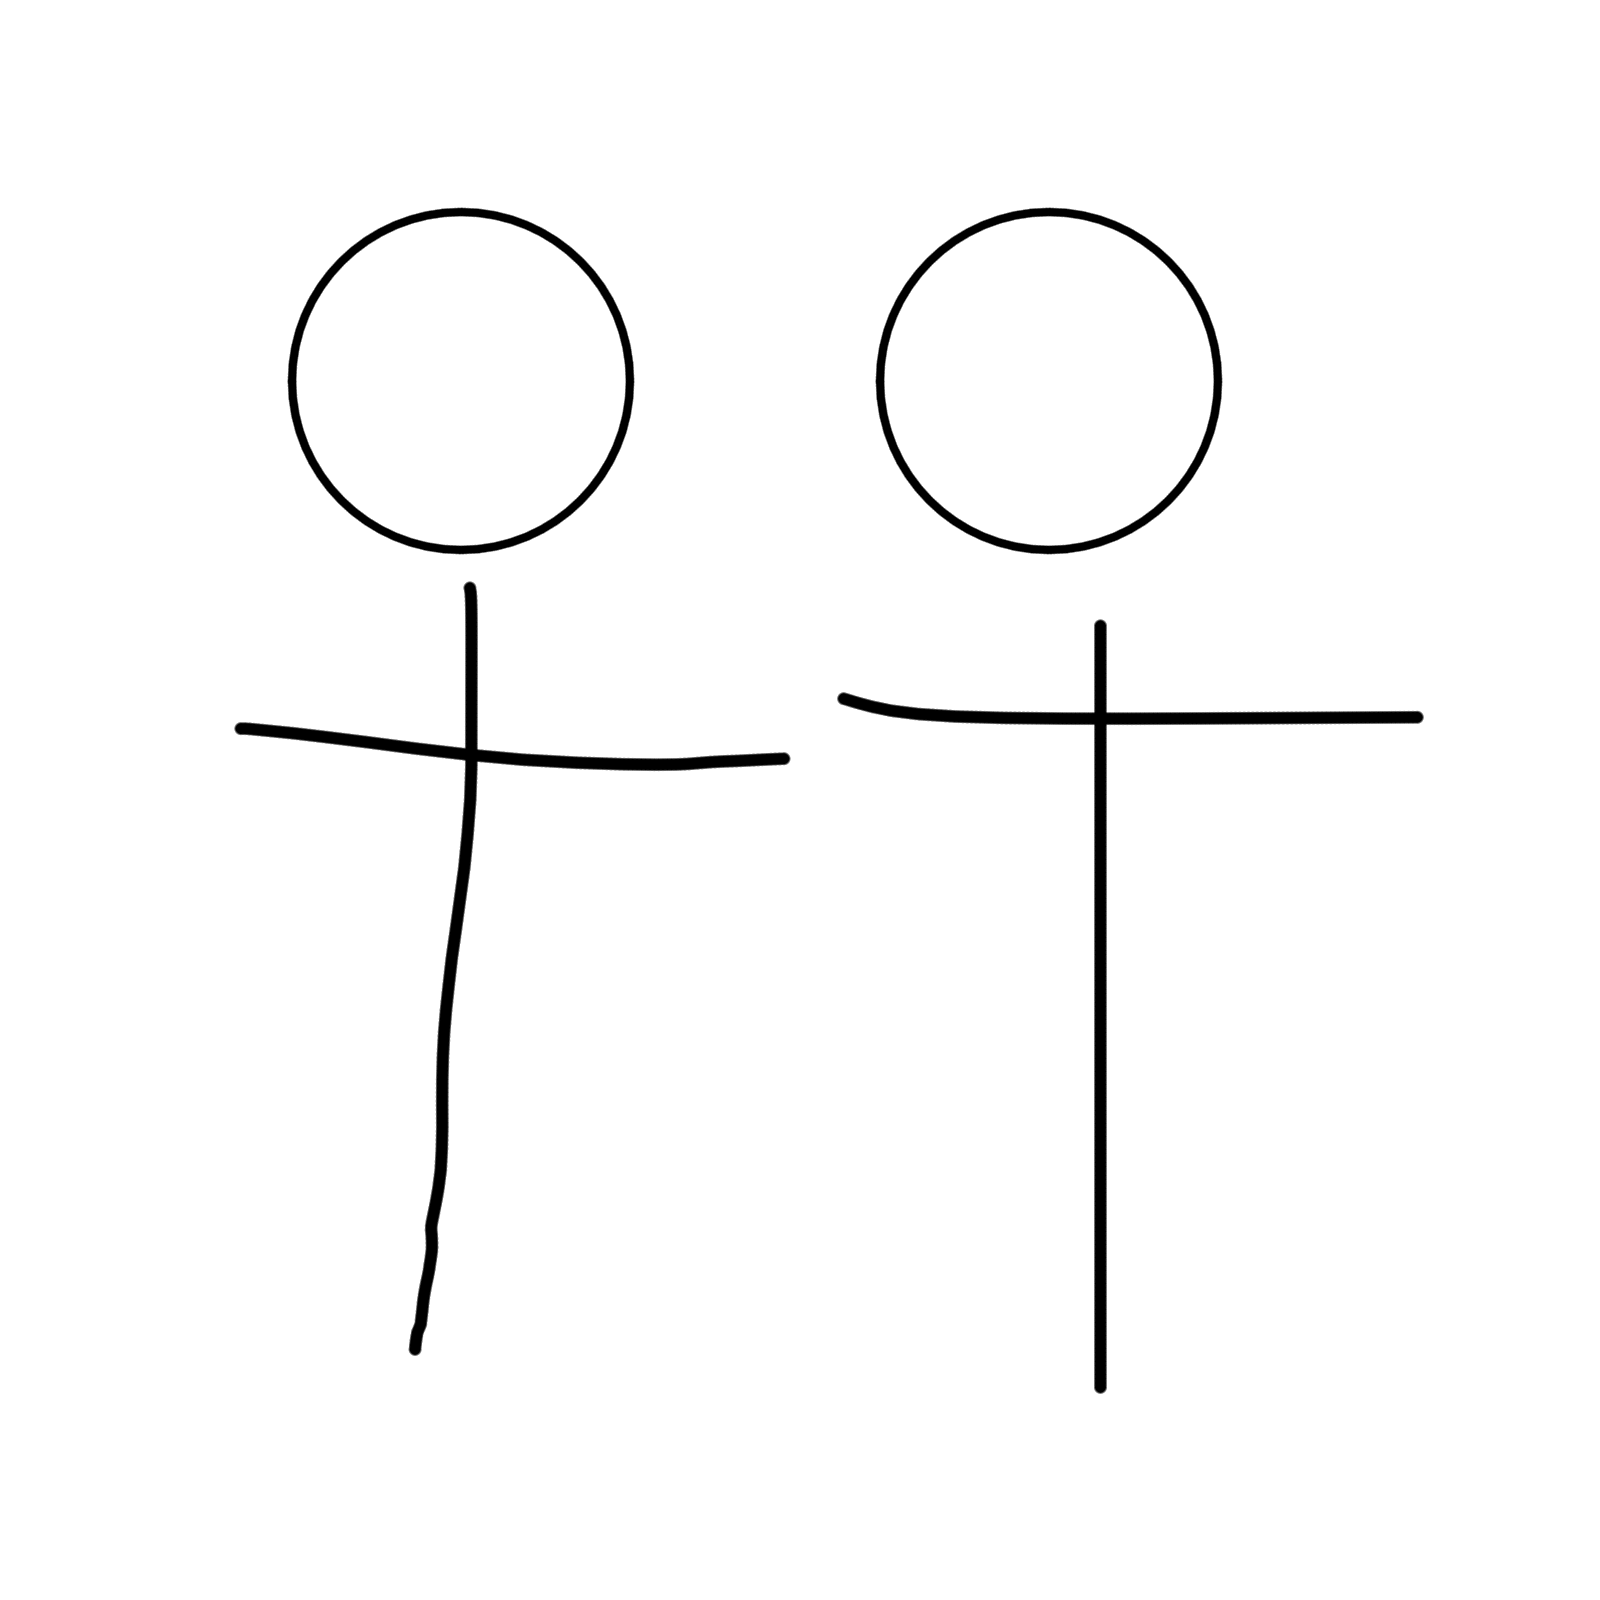
\includegraphics[width=\linewidth, height=20mm]{img/4-1loa_separate_keyframe}
    \end{minipage}
    & & & 
    \\ \hline
    5 LOA 
    &
    \begin{minipage}{.15\textwidth}
      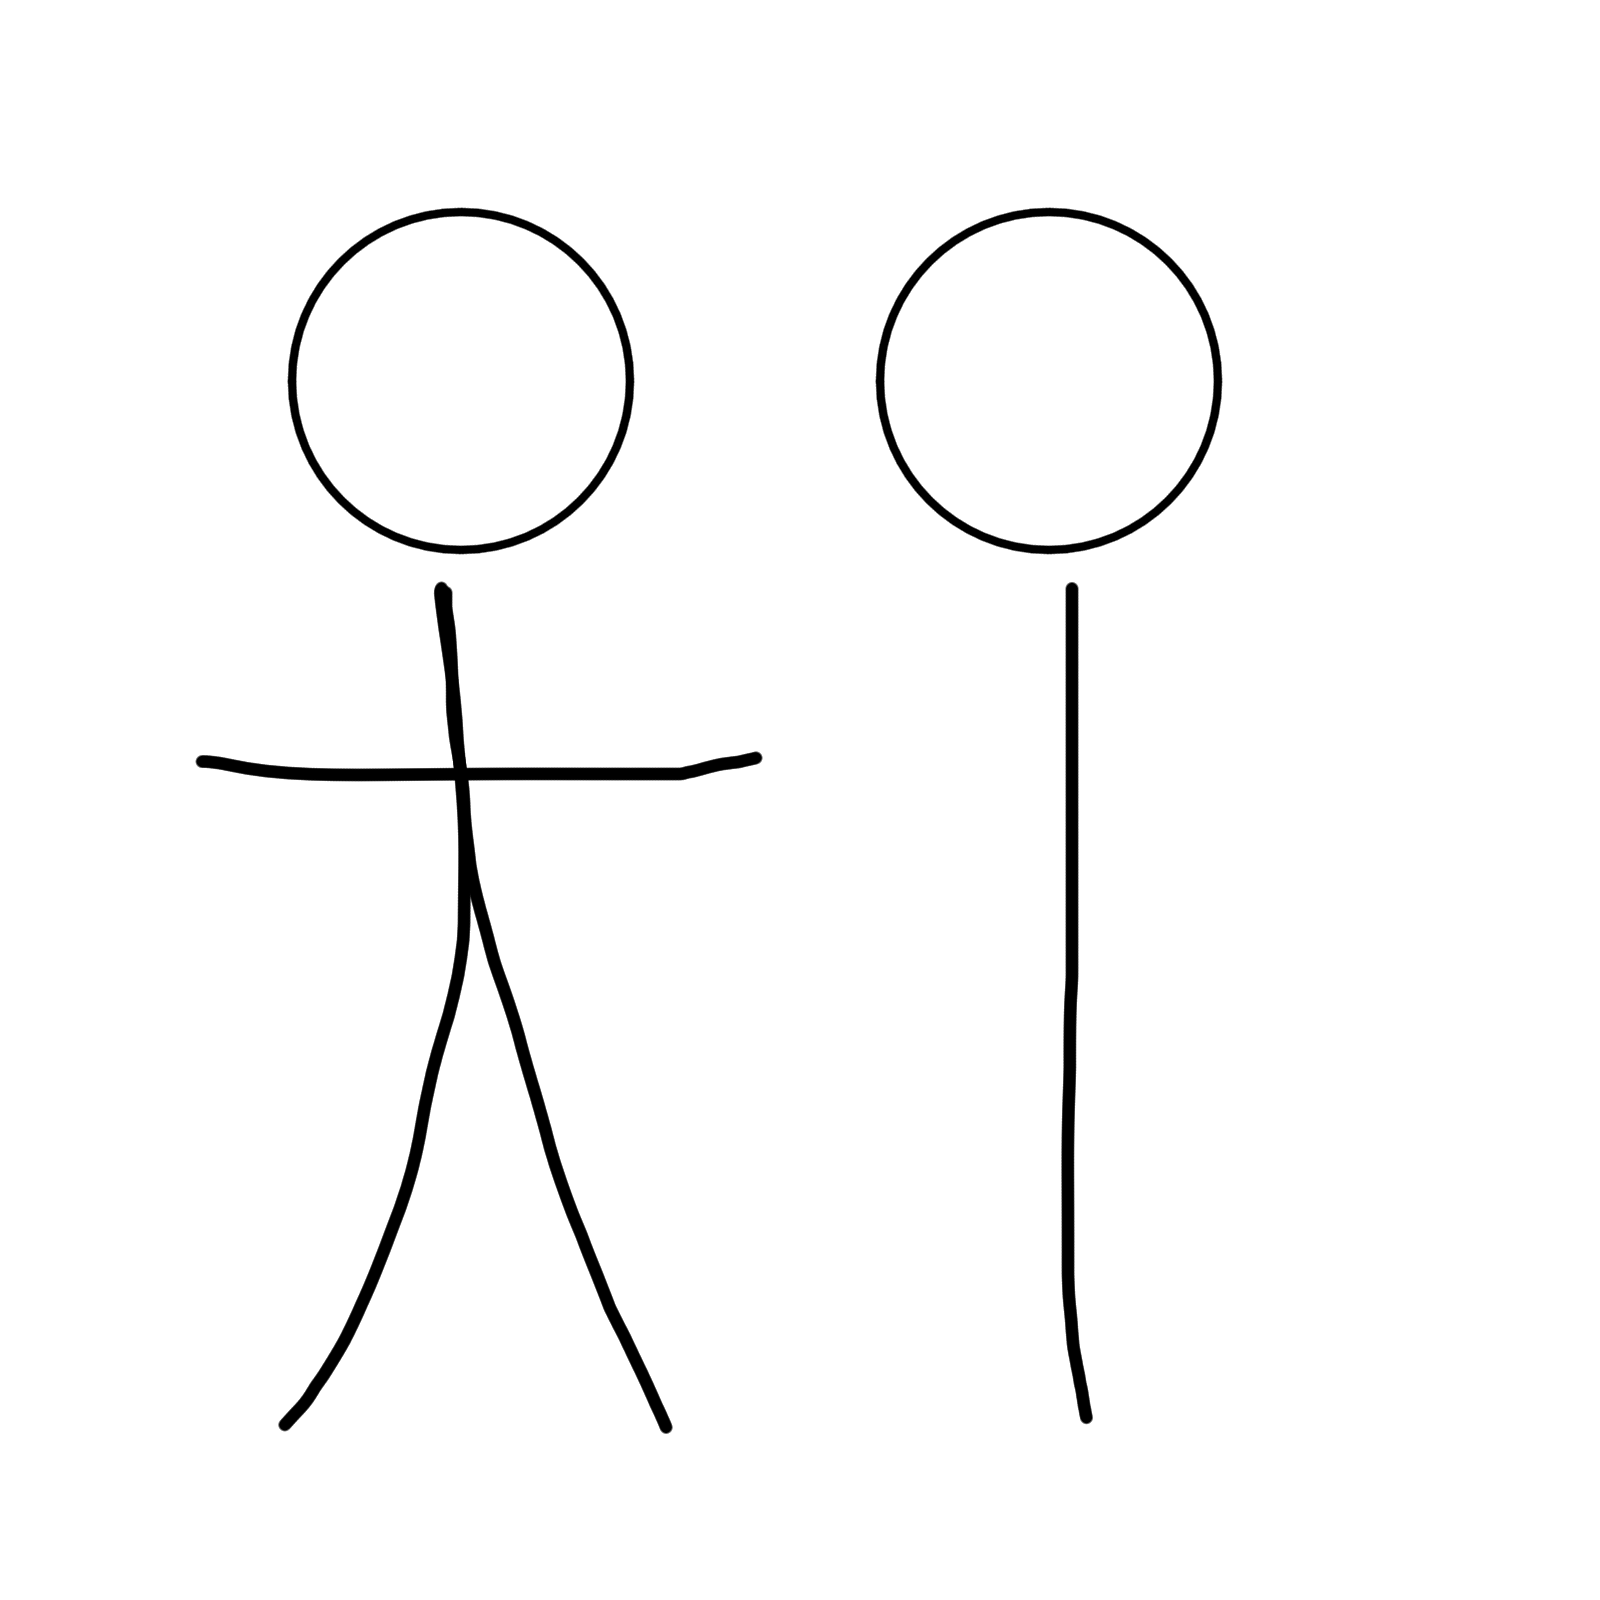
\includegraphics[width=\linewidth, height=20mm]{img/5loa_separate_keyframe}
    \end{minipage}
    &
    \begin{minipage}{.15\textwidth}
      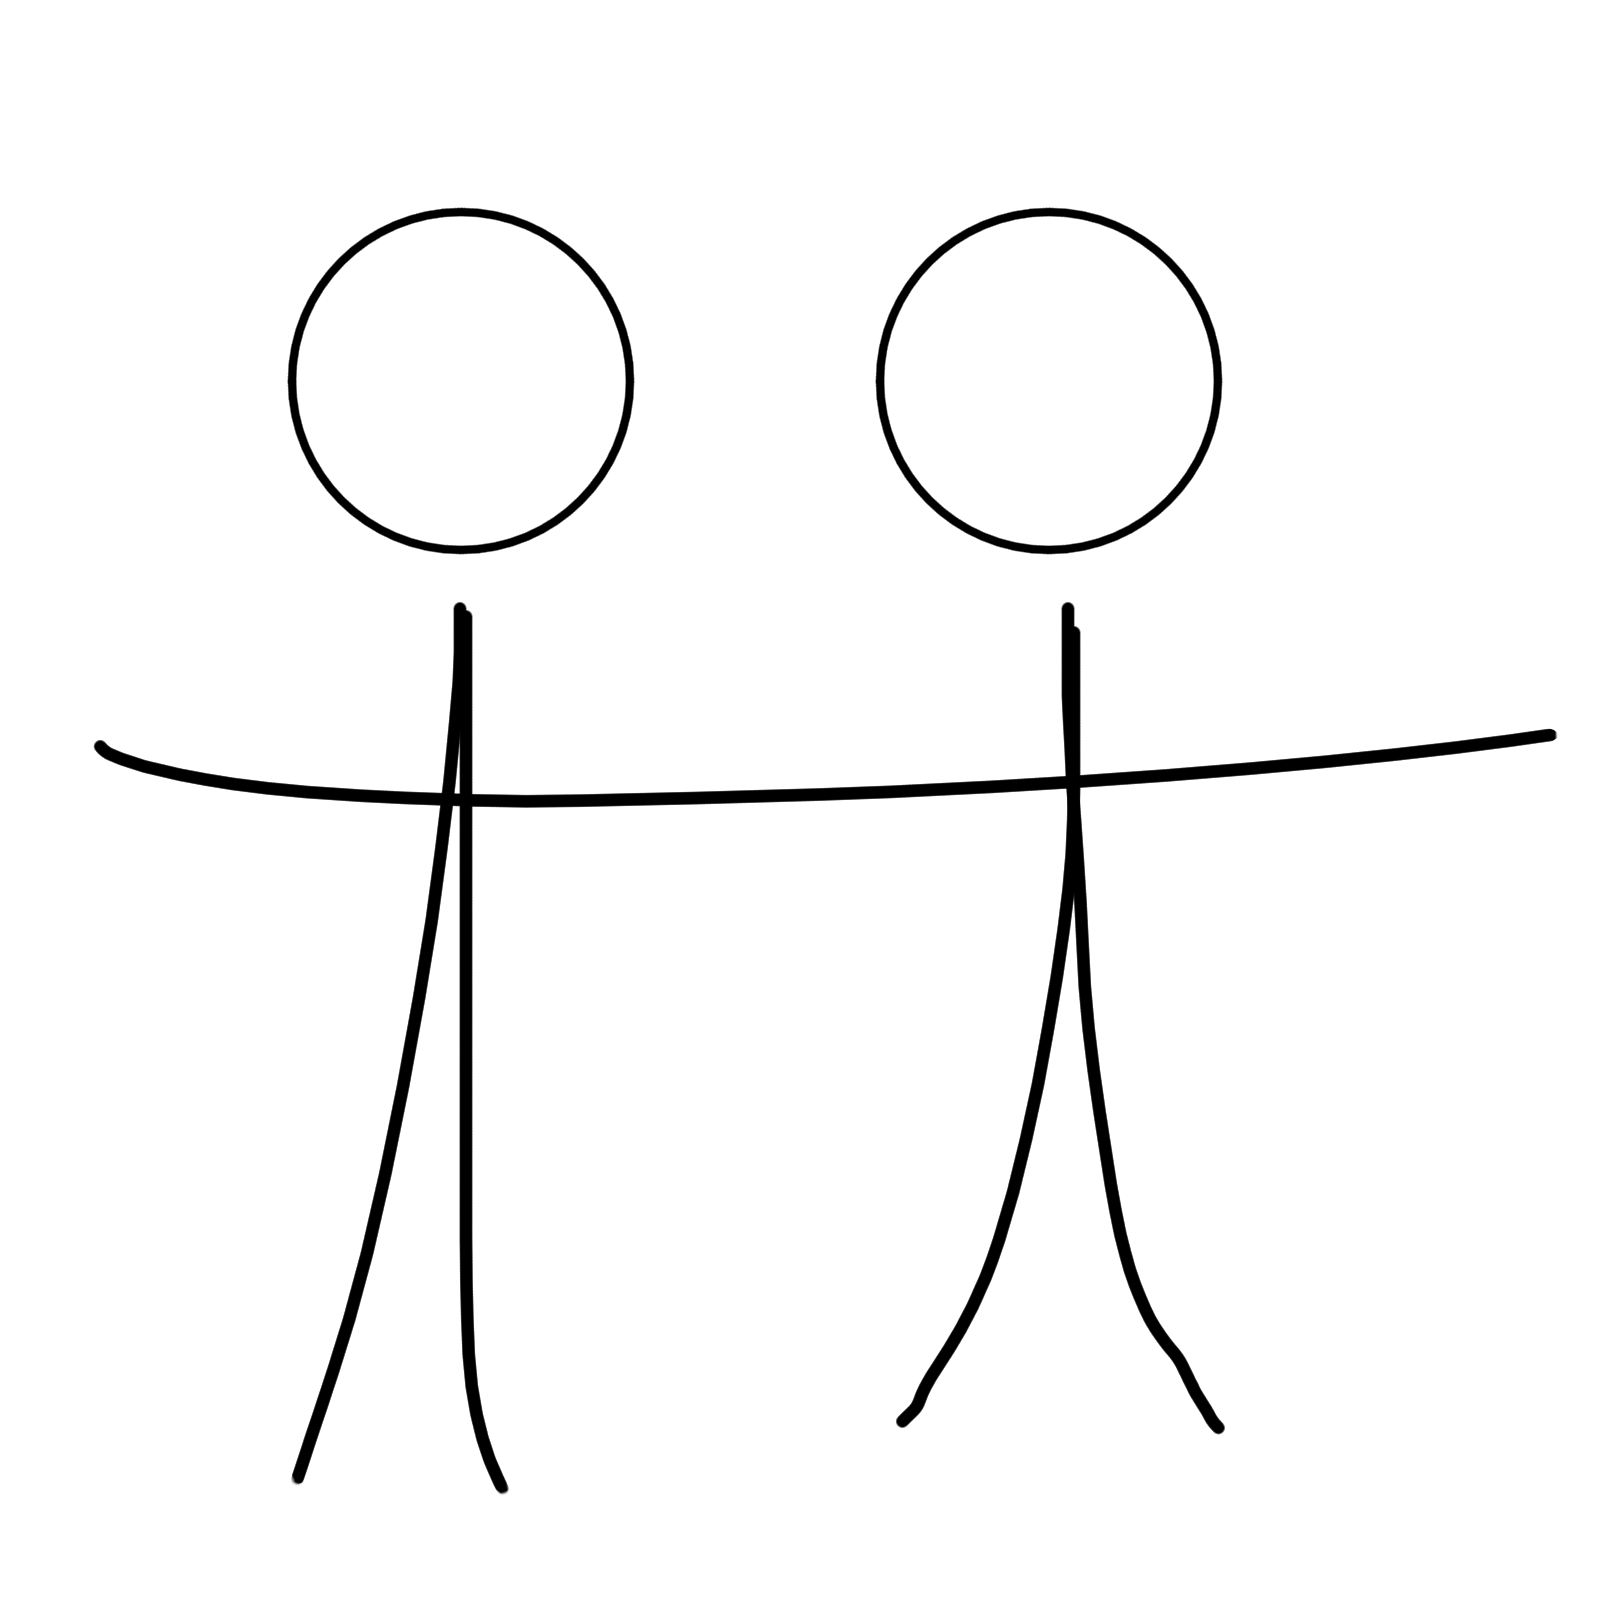
\includegraphics[width=\linewidth, height=20mm]{img/10keyframe}
    \end{minipage} & & 
    \\ \hline
    6 LOA 
    &
    \begin{minipage}{.15\textwidth}
      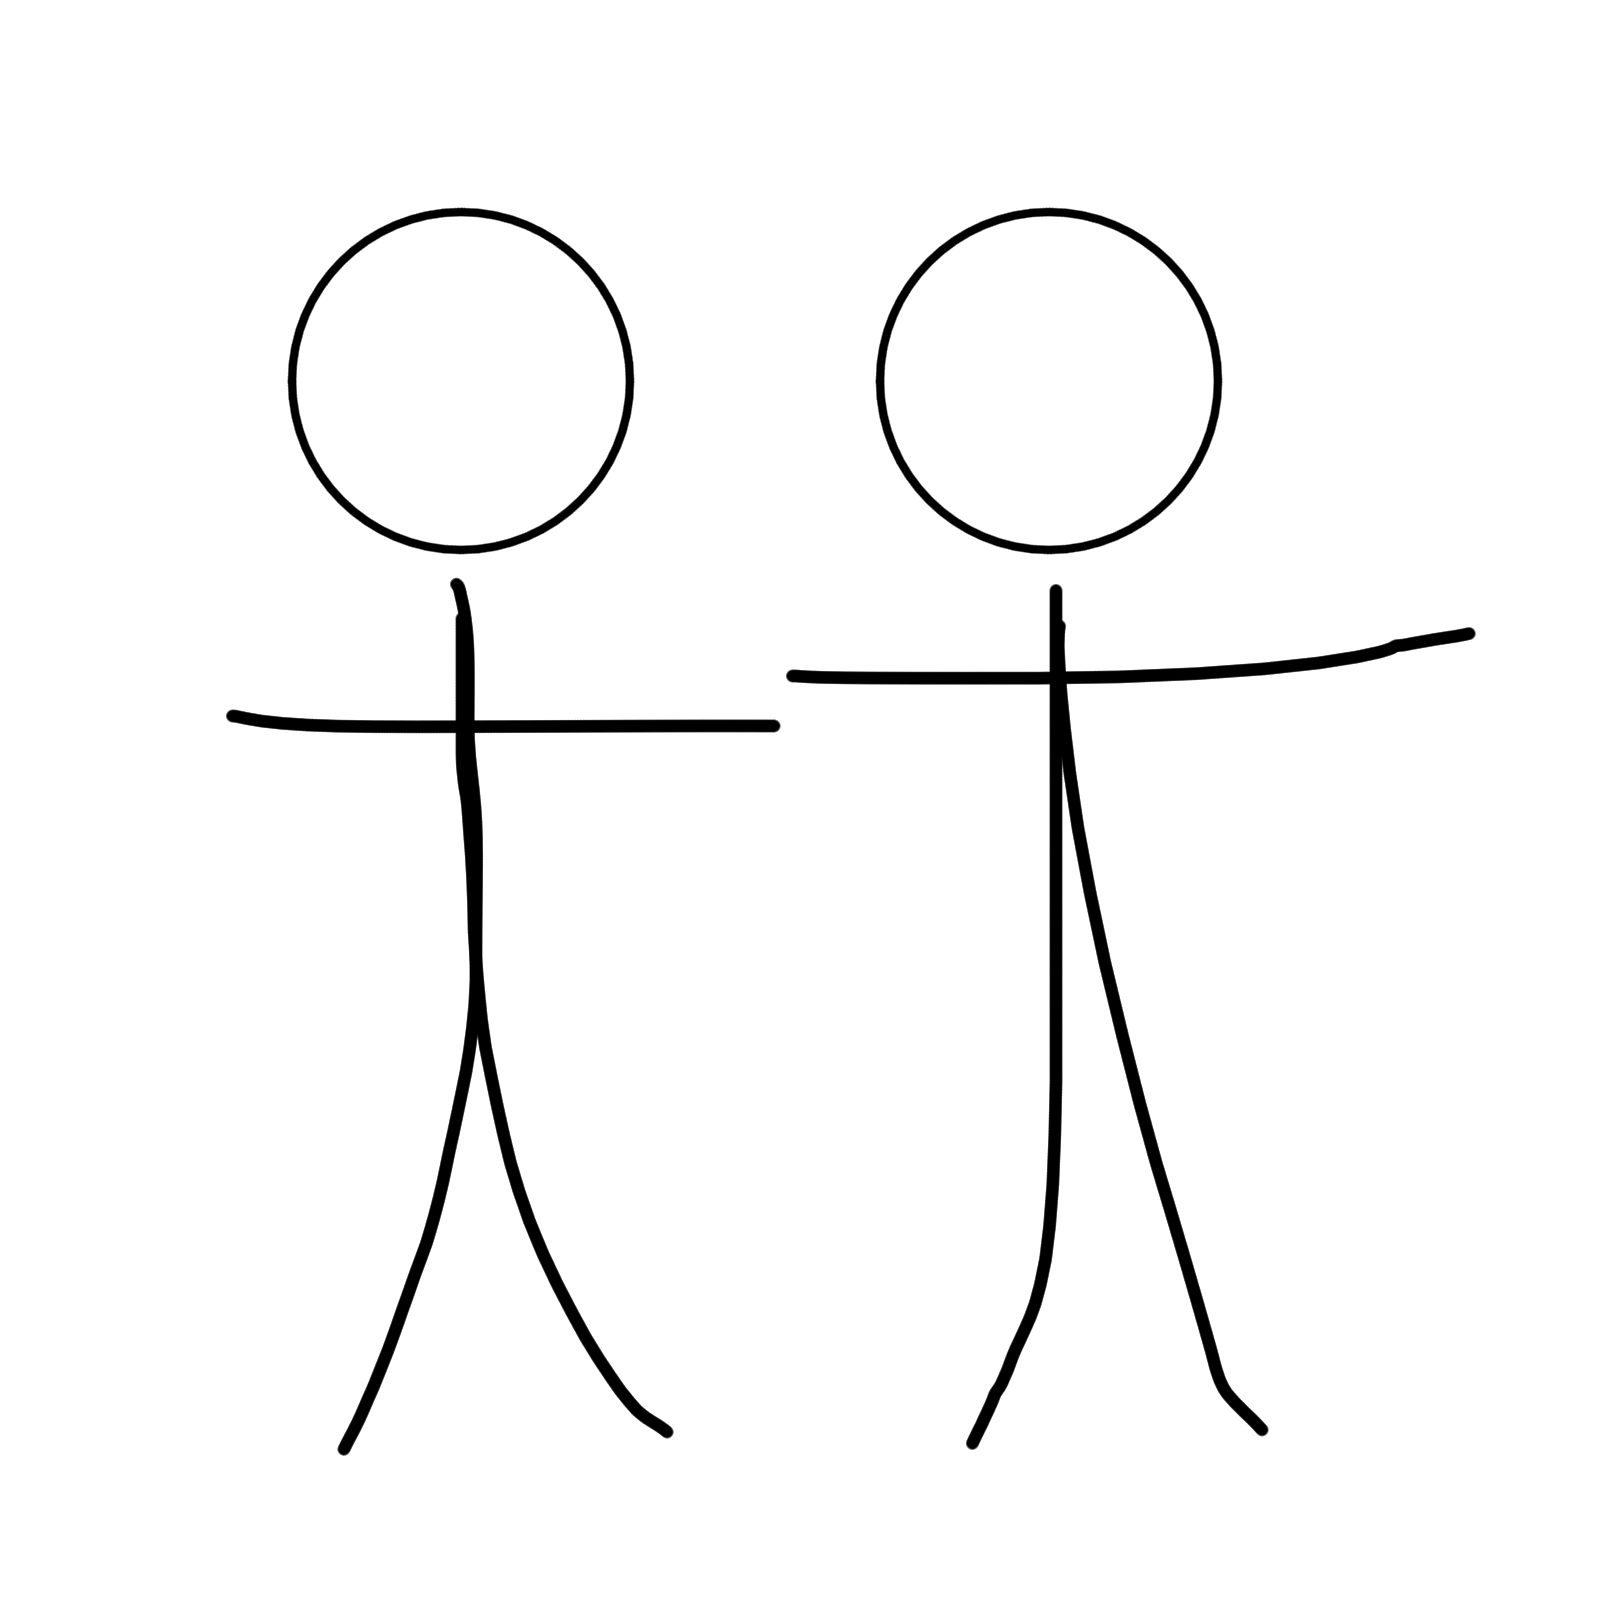
\includegraphics[width=\linewidth, height=20mm]{img/6loa_separate_keyframe}
    \end{minipage}
    & & & 
    \\ \hline
  \end{tabular}
  \caption{Types of Keyframes for Two Dancing Characters}
  \label{table:LOAChart}
\end{table}


\section{User Constraints}
Only allowed to connect and disconnect skeletons at keyframes.
